\documentclass[11pt,twoside]{article}

\usepackage{paperlighter}

% Recommended, but optional, packages for figures and better typesetting:
\usepackage{microtype}
\usepackage{graphicx}
\usepackage{subfigure}
\usepackage{booktabs} % for professional tables

% Attempt to make hyperref and algorithmic work together better:
\newcommand{\theHalgorithm}{\arabic{algorithm}}


% For theorems and such
\usepackage{amsmath}
\usepackage{amssymb}
\usepackage{mathtools}
\usepackage{amsthm}

% if you use cleveref..
\usepackage[capitalize,noabbrev]{cleveref}

%%%%%%%%%%%%%%%%%%%%%%%%%%%%%%%%
% THEOREMS
%%%%%%%%%%%%%%%%%%%%%%%%%%%%%%%%
\theoremstyle{plain}
\newtheorem{theorem}{Theorem}[section]
\newtheorem{proposition}[theorem]{Proposition}
\newtheorem{lemma}[theorem]{Lemma}
\newtheorem{corollary}[theorem]{Corollary}
\theoremstyle{definition}
\newtheorem{definition}[theorem]{Definition}
\newtheorem{assumption}[theorem]{Assumption}
\theoremstyle{remark}
\newtheorem{remark}[theorem]{Remark}

% Todonotes is useful during development; simply uncomment the next line
%    and comment out the line below the next line to turn off comments
%\usepackage[disable,textsize=tiny]{todonotes}
\usepackage[textsize=tiny]{todonotes}

\usepackage{xcolor}
\usepackage{listings}
\lstset{basicstyle=\ttfamily,
  showstringspaces=false,
  commentstyle=\color{red},
  keywordstyle=\color{blue},
  numbers=left, numberstyle=\scriptsize
}

%\usepackage[T1]{fontenc}




\usepackage[square,numbers]{natbib}




\slimtitle{Kaldi Tedlium s5\_r3 Writeup}
\slimauthor{Sourya Kakarla}


\begin{document}

\lightertitle{Kaldi Tedlium s5\_r3 Pipeline Writeup}

\lighterauthor{Sourya Kakarla (sk5057)}

%\lighteremail{xxx@xxx.com}


%\begin{abstract}
Using \LaTeX{} to write papers is concise and convenient. However, for writing in life, complicated \LaTeX{} style-files (e.g., elegantpaper) are difficult to access, or submission style-files (e.g., journal or conference) are not free indeed. To tackle these problems and satisfy an elegant and straightforward scientific writing, \textbf{paperlighter.sty}, a one-column style-file, is designed. This document is edited from icml2022.sty and provides a basic paper template. Compared to icml2022.sty, paperlighter.sty contain fewer operations, reducing adjustment while keep graceful. \textbf{\textit{Notably, the paper's main content only describes the format of icml2022.sty. We place the content to show the actual effect of paperlighter.sty.}}
\end{abstract}


\section{Introduction}


%cmd.sh

%decode_nj - decoding is very expensive
%comment out most of the decoding
%only in last stage

%nj : number of jobs is related to number of processors 4 or 8

%Staging allows you to start from where you left off by setting the stage variable

%train_rnnlm : Should script train a language model using a RNN. Most cases you just want to download the RNNLM for rescoring.
%should it train the rnnlm

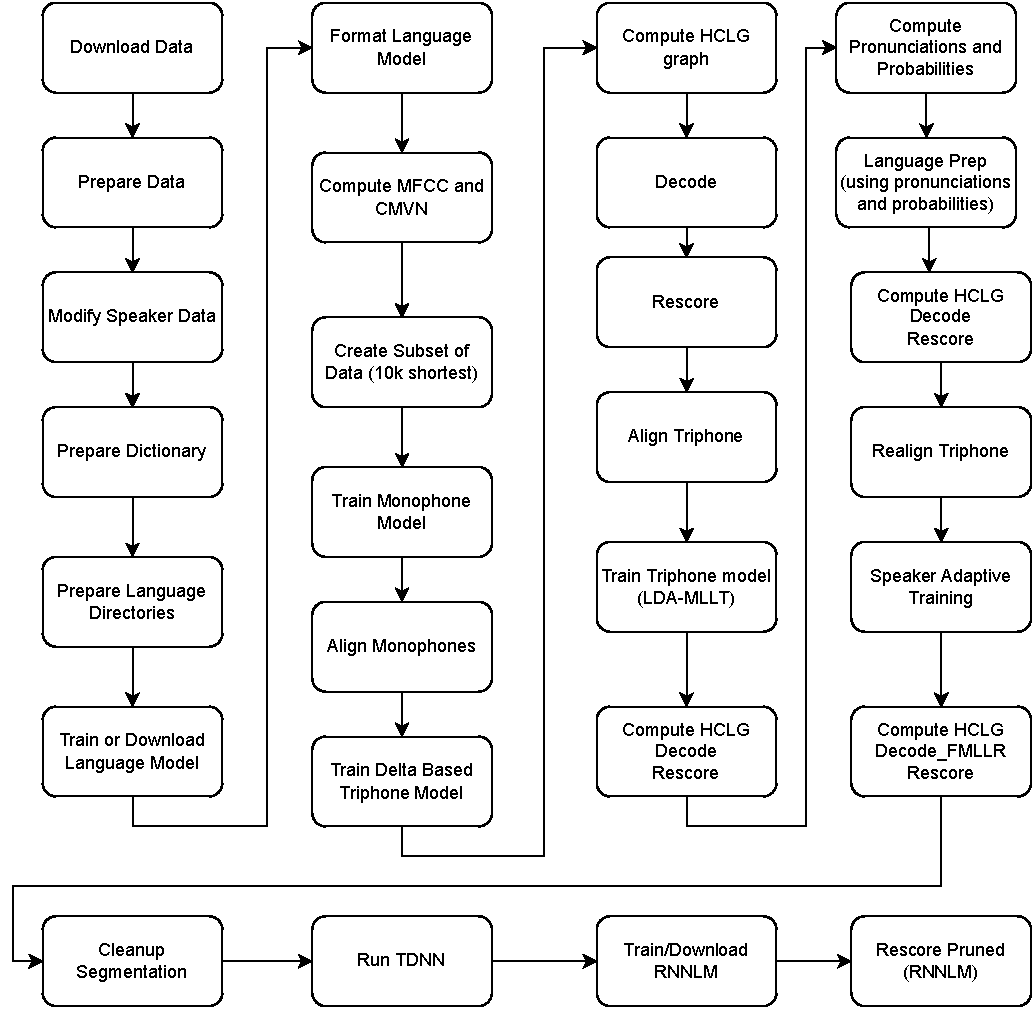
\includegraphics{figure/Kaldi.drawio.pdf}

%stm file format


\section{Stages}
\subsection{Stage 0 - Download TEDLIUM release-3 data}
In this stage, the \path{local/download_data.sh} script is run to download the Tedlium dataset \href{http://www.openslr.org/resources/51/TEDLIUM_release-3.tgz }{from OpenSLR} using \texttt{wget}.
The downloaded \path{TEDLIUM_release-3.tgz} is saved in the \texttt{db/} folder and extracted there.
After downloading the data, \path{download_data.sh} finally validates the number of \texttt{.sph} files in the \path{TEDLIUM_release-3/data/} directory. The expected count is $2351$ if everything goes well.

\subsection{Stage 1 - Prepare Data}

In this stage, processing on the data downloaded in Stage 0 is done by running the script \path{prepare_data.sh} and files of different kinds are generated for the dev, test, and train partitions which will be used in the later stages as part of language model training and so on.
They are as follows:
\begin{itemize}
    \item \texttt{text}: Contains mappings between utterances (transciptions) and utterance ids which will be used by Kaldi
    \item \texttt{segments}: Contains mappings between \texttt{utterance-id} and segment of a particular recording. It contains the start and end times for each utterance in an audio file. It is of the format 
    \texttt{utt\_id file\_id start\_time end\_time} ~\cite{kalditut}.

    \item \texttt{utt2spk }: One-to-one mapping between utterance ids and the corresponding speaker identifiers. 
    \item \texttt{spk2utt}: Mapping between the speaker identifiers and all the utterance identifiers associated with the speaker recording. 
    \item \texttt{wav.scp}: A list of Utterances to Filenames with each line of format \path{<recording_id> <extended_filename>}
    \item \texttt{reco2file\_and\_channel}: Used when scoring (measuring error rates) with NIST's \emph{sclite} tool.
    \item \texttt{glm}: An empty glm file is generated.
\end{itemize}

As part of the processing, silence is padded to the segments, especially at the beginning.
Further, the speakers are split into 3-minutes chunks by running the \texttt{utils/data/modify\_speaker\_info.sh}
The generated files are validated to check if they meet Kaldi's format specifications.



\subsection{Stage 2 - Prepare Dictionary}
In this stage, \path{prepare_dict.sh} script is run to create the files at \path{data/local/dict_nosp} required downstream for the language model.
The main steps in this stage are as follows:
\begin{itemize}
    \item Processing is done on the \path{db/TEDLIUM_release-3/TEDLIUM.152k.dic} dictionary by ignoring instances of \texttt{<unk>}, entries with numbers, and sorting alphabetically to create the \path{data/local/dict_nosp/lexicon_words.txt}.
    
    \item Files are created for non-silent phones (\path{data/local/dict_nosp/nonsilence_phones.txt}) and silent phones respectively (\path{data/local/dict_nosp/silence_phones.txt}). The silent phones are \texttt{SIL} (silence) and \texttt{NSN} (non-spoken noise).
    
    \item \path{optional_silence.txt} is generated which simply contains an \texttt{SIL} model.
    \item \path{data/local/dict_nosp/lexicon.txt} is created by taking unique entries from \texttt{lexicon\_words.txt} and adding the silence (\texttt{SIL}) and noise (\texttt{NSN}) phones to them. The lines in the \texttt{lexicon.txt} are in the format of \texttt{word phone1 phone2...phoneN}
\end{itemize}

\subsection{Stage 3 - Pepare Language Files}
In this stage, the \path{utils/prepare_lang.sh} script is run with following parameters as input
\begin{itemize}
    \item \path{data/local/dict_nosp} (dictionary source directory)
    \item \path{<unk>} (lexical entry for uknown)
    \item \path{data/local/lang_nosp} (temporary directory for processing)
    \item \path{data/lang_nosp} (target language directory)
\end{itemize}

It prepares the \texttt{data/lang\_nosp/} directory in the Kaldi standard format which contains the following files and folders. \texttt{nosp} refers to the model before computation of silence probabilities and pronunciation.
\begin{itemize}
    \item \texttt{G.fst}: Finite State Transducer form of the language model.
    \item \texttt{L.fst}: Finite State Transducer form of the lexicon .
    \item \path{L_disambig.fst}: The lexicon, as above but including the disambiguation symbols \#1, \#2, and so on, as well as the self-loop with \#0 on it to "pass through" the disambiguation symbol from the grammar.
    \item \texttt{oov.txt}: Contains a single line of the format \texttt{<unk>} which is the word to which all out-of-vocabulary words map to during training.
    \item \texttt{oov.int}: Integer form of the above (\texttt{38}).
    \item \texttt{phones/}: Directory containing various files regarding the phone set. Most of the files exist in 3 separate versions - \texttt{txt}, \texttt{int}, and \texttt{csl}.
    \item \texttt{phones.txt}: Symbol-table file, in the OpenFst format, where each line is in the text form and integer form. Example: \texttt{T\_E 132}. Used by Kaldi to map back and forth between the integer and text forms of these symbols.
    \item \texttt{words.txt}: Similar to \texttt{phones.txt} but for words. Example: \texttt{arsenal 7054}.
    \item \texttt{topo}: Specifies the topology of the HMMS used.
\end{itemize}

All the generated files are validated using \path{utils/validate_lang.pl} script.

\subsection{Stage 4 - Train or Download Language Model}
Depending upon the \path{train_lm} variable in \texttt{run.sh}, this stage trains a language model by running the \path{ted_train_lm.sh} script which trains a language model using the TEDLIUM 6 data sources if \path{train_lm} is set to \texttt{true} or runs \path{ted_download_lm.sh} to download ARPA-style 4-gram language models (arpa.gz) from \url{kaldi-asr.org} if otherwise. By default, \path{train_lm} is set to \texttt{fasle}.

In the \path{ted_train_lm.sh} script, the training is does on Cantab-Tedlium text data and tedlium acoustic training data which from the earlier stages.
It is based on the example scripts that come with PocoLM~\cite{pocolm} and creates models in the ARPA format~\cite{arpaformat}.

%explaination about ted_train_lm if possibles




\subsection{Stage 5 - Format Language Model}

In this stage, the \texttt{format\_lms.sh} script is run to generate certain language models in suitable formats as follows:
\begin{itemize}
    \item The script checks for the existence of \texttt{data/lang\_nosp/G.fst} and if not available, creates it by converting the ARPA-format language model \path{4gram_small.arpa.gz} into an OpenFST format using \texttt{arpa2fst}~\cite{arpa2fst} which is a Kaldi program that turns the ARPA-format language model into a Weight Finite State Transducer. Further, it verifies if \texttt{G.fst} is stochastic enough using \texttt{fstistochastic}.
    \item It checks for the \texttt{data/lang\_nosp/G.carpa} and if not available, creates it by converting the ARPA-format language model \path{4gram_big.arpa.gz} into a ConstArpaLm~\cite{constarpa}  format model by running the script \path{utils/build_const_arpa_lm.sh }. This model is used downstream for rescoring.
\end{itemize} 
 It also performs a series of checks on the encoding of all the files in \path{data/lang_nosp/} directory using the \path{utils/validate_lang.pl} script.
%cite https://kaldi-asr.org/doc/data_prep.html
\subsection{ Stage 6 - Feature Extraction }


In this stage, MFCC features are extracted for all the 3 data partitions (test, dev, and train) 
using the \texttt{steps/make\_mfcc.sh} script on the data placed in the \texttt{data/<\$set>} 
($\$set = {test,dev,train}$) directories. It uses the \texttt{compute-mfcc-feats} command-line tool
to produce the required MFCC features. A broad overview~\cite{mfcc} of the MFCC feature extractions is as follows:
\begin{itemize}
    \item Work out the number of frames in the file (typically 25 ms frames shifted by 10ms each time).
    \item For each frame: 
        \begin{itemize}
         \item Extract the data, do optional dithering, preemphasis and dc offset removal, and multiply it by a windowing function.
         \item Calculate the energy (negative log), do FFT and compute the power spectrum.
         \item Compute log of the energy in each mel bin and take cosine transform keeping the required number of coefficients.
        \end{itemize}
\end{itemize}
Further, cepstral mean and variance statistics (CMVN)~\cite{kaldicmvn} per speaker are computed for all the 3 data partitions using the \path{steps/compute_cmvn_stats.sh} script which helps in compensation of noise and reduces mismatch between different data partitions.
\subsection{ Stage 7 - Select 10k Shortest Utterances }
In this stage, 10k shortest utterances are selected using the \path{utils/subset_data_dir.sh}
script from the \texttt{data/train} directory and put in \path{data/train_10kshort}. Further, excessive repetitions of utterances are eliminated if they occur more than a particular number of times (10) and output is placed in \path{ data/train_10kshort_nodup} directory by running the \path{remove_dup_utts.sh} with the maximum allowed number of repetitions as 10. The number of utterances drop to 9135 from 10000. This subset creation is useful for monophone training downstream.


\subsection{ Stage 8 - Monohpone Model Training  }
In this stage, the monophone models are trained using the \path{train_mono.sh} script on the \path{data/train_10kshort_nodup.sh} (generated in the previous stage) and \path{data/lang_nosp} and are saved in the \texttt{exp/mono/} directory. 

This is the primary step of the actual training process in the pipeline. The smaller subset of 10k utterances is used to achieve efficiency. Even with little data, satisfactory monophone models can be trained and are used to bootstrap training for later models in the upcoming stages.

The monophone model is a purely acoustic model and does not include any contextual information about the adjacent phones. It is the building block for the models which have context embedded into them (such as the triphone in the next stage).


%steps/diagnostic/analyze_alignments.sh --cmd run.pl data/lang_nosp exp/mono

\subsection{ Stage 9 - Align Monophones and Train delta-based triphones  }
By running the script \path{align_si.sh}, data in \path{data/train} is aligned using model (through deltas) from \path{exp/mono/} and the alignments are put in \path{exp/mono_ali}. Further, delta-based triphones are trained using the language model \path{data/lang_nosp} and  monophone alignments \path{mono_ali} and are placed in the \path{exp/tri1/} directory.

Even though the parameters of the acoustic model are estimated in the monophone model training in the previous stage, the aim is to improve it in this stage using contextual information, thus the triphones. Viterbi training is used to achieve this. By aligning the audio to the transript from the training data with the most current acoustic model, training algorithms use this to improve the parameters of the model. 


As only a small subset of all triphone possibilites are actually relevant for the model, phonetic decision tree groups are used to classify the phones into a minimal set of acoustically distinct units, thus reducing the number of parameters.

Consequently, each training step is followed by an alignment step so that the audio and the text can be realigned.





\subsection{ Stage 10 - Decoding and Rescoring}
A fully expanded decoding graph (HCLG.fst model) is computed at \path{exp/tri2/graph_nosp} by running \path{utils/mkgraph.sh} that represents the language-model, lexicon, context-dependency, and HMM structure in the model. HCLG = H o C o L o G~\cite{decodinggraph}.

\begin{itemize}
    \item G is an acceptor (i.e. its input and output symbols are the same) that encodes the grammar or language model.
    \item L is the lexicon; its output symbols are words and its input symbols are phones.
    \item C represents the context-dependency: its output symbols are phones and its input symbols represent context-dependent phones, i.e. windows of N phones.
    \item H contains the HMM definitions; its output symbols represent context-dependent phones and its input symbols are transition-ids, which encode the pdf-id and other information. 
\end{itemize}

After the HCLG graph is calculated, decoding the utterances using the graph is done by running \path{steps/decode.sh} on the graph at \path{exp/tri2/graph_nosp} and WERs are calculated using \path{lmrescore_const_arpa.sh} which rescores the lattices with ConstArpaLm format language model.
\subsection{ Stage 11 - Align delta-based triphones and Train (LDA-MLLT)}
Similar to the first part of Stage 9, triphones are aligned by running the \path{align_si.sh} , the difference being \path{exp/tri1/} being the input model and output alignments placed in \path{exp/tri1_ali}.

A triphone model with LDA (Linear Discriminant Analysis)~\cite{kaldilda} and MLLT (Maximum Likelihood Linear Transform)~\cite{kaldimllt} feature transforms is trained using the training alignments obtained from above (\path{exp/tri1_ali}) by running the \path{steps/train_lda_mllt.sh} script and the new model is placed in \path{exp/tri2} directory.


\subsection{ Stage 12 - Decoding and Rescoring Updated Triphone Model}
This stage is identical to Stage 10 except for that the decoding and rescoring is done using the latest model (\path{exp/tri2/}) from Stage 11.
\subsection{ Stage 13 - Compute Pronunciations and Probabilities}
Linear lattices are computed for each utterance in the training data \path{data/train/} by using the latest alignment \path{exp/tri2} and language model \path{data/lang_nosp/} by running the script \path{steps/get_prons.sh}.

A lattice is a representation of the alternative word-sequences that are "sufficiently likely" for a particular utterance~\cite{kaldilattice}. Files of the form \path{prons.*.gz} are generated and the various counts of pronunciations are computed which are used in the next step in this stage.

Next, by running the \path{utils/dict_dir_add_pronprobs.sh} on the counts obtained from above, a modified dictionary directory with pronunciation probabilities is computed in \path{data/local/dict/}, for example \path{data/local/dict/lexiconp.txt} and \path{data/local/dict/lexiconp_silprob.txt} which includes the silence probabilities as well.
\subsection{ Stage 14 - Language Prep, Decoding, and Rescoring}
The first step in this stage is similar to Stage 3 except that \path{data/local/dict/} is used to generate the files at \path{data/lang/} (as opposed to \path{data/lang_nosp/})  as the dictionary source directory as we now have the probabilities.

The decoding graph is now recomputed in \path{exp/tri2/graph/} using the new language files at \path{data/lang/} and decoding is done as before. Rescoring is done to evaluate the performance of the upgraded language model.

\subsection{ Stage 15 - Realign Trihpones and Speaker Adaptive Training (SAT) }
The tirphone alignments are recomputed using the latest language files (with pronunciation probabilities) from the previous stage.

Next, Speaker Adaptive Training is done by running \path{steps/train_sat.sh} using the latest language model and alignments and a new triphone model is generated at \path{exp/tri3/}. SAT performs speaker and noise normalization by adapting to each speaker with a particular data transform resulting in more homogeneous data. This allows the model to be phoneme based than speaker and/or environment based.

In this stage, the decoding step has a significant alteration. The script \path{steps/decode_fmllr.sh} is run for the decoding after the graph creation as opposed to \path{steps/decode.sh} in the previous stages. This script uses feature-space MLLR (fMLLR)\cite{fmllr} transform for the first time in this recipe for speaker adaptive decoding.

Finally rescoring is done using the lastest model and outputs from the fMLLR decoding.
\subsection{ Stage 16 - Cleanup Segmentation}
The segmentation done earlier is improved by running the script \path{run_cleanup_segmentation.sh} which re-segments the training data by selecting only "good" audio that matches the transcripts.

In running the script, \path{steps/cleanup/clean_and_segment_data.sh} script is used to clean the training data based on the acoustic and language models trained so far.

Next, updated alignments are computed using the \path{steps/align_fmllr.sh} script. Further, Speaker Adaptive Training is redone with latest segmentations.
Finally decoding (fMLLR) and rescoring is like in the previous stage.
\subsection{ Stage 17 - Run Time Delayed Neural Network}
In this stage, the \path{tuning/run_tdnn_1d.sh} script is run to train a TDNN model to learn acoustic features on the latest data.

First, i-Vector extraction is done by running the \path{run_ivector_common.sh} script. An iVector is a vector of dimension several hundred (one or two hundred, in this particular context) which represents the speaker properties~\cite{ivector}. As part of the extraction, data augmentation is done, and speed-perturbed data is prepared from that~\cite{understandingkaldi}. Next, MFCC and CMVN of the speed-perturbed data is computed. Finally training alignments of the speed-perturbed data are obtained. Volume perturbation is then done on speed-perturbed train dataset. High-resoultion MFCCs and CMVNs are extracted from the volume and speed perturbed data.

The \path{steps/nnet3/chain/gen_topo.py} script is run to populate the \path{data/lang_chain/} directory with a chain topology~\cite{chaintop}. This topology is used for Kaldi nnet3 DNN-HMM models.

Next alignments and lattices are obtained from low resoultion MFCCs by running \path{steps/align_fmllr_lats.sh}.

Next a new decision tree is built using lowe-resolution MFCCs, the new topology and alignments by running \path{steps/nnet3/chain/build_tree.sh}

A config file for the DNN sturcture is built using \path{steps/nnet3/xconfig_to_configs.py }

The configured DNN is trained using the high-resolution MFCCs, new decisions tree and i-vectors extracted in the previous steps by running \path{steps/nnet3/chain/train.py}.

Finally graph is recomputed (using \path{utils/mkgraph.sh}), decoding and rescoring are done similar to the previous stages.
\subsection{ Stage 18 - Download or Run RNNLM}
Based on the variable \path{train_rnnlm}, a language model is downloaded (if \texttt{False}) using \path{local/ted_download_rnnlm.sh} or a Recurrent Neural Network Language Model is trained locally by running the 
\path{local/rnnlm/tuning/run_lstm_tdnn_a.sh} and \path{local/rnnlm/average_rnnlm.sh} scripts. A RNN language model is better performing than an n-gram model as it deals well with the sparseness. 

After necessary preparation and configuration steps, it is by running \path{rnnlm/train_rnnlm.sh} script the model is first trained. Later, \path{average_rnnlm.sh} script takes the default \path{rnnlm_dir} of the recipe and averages the best model and the 10 previous and following ones (if they exist).

\subsection{ Stage 19 - Rescore Lattices (Pruned Algorithm)}
This is the last stage of the pipeline. The script \path{rnnlm/lmrescore_pruned.sh} is run to rescore lattices with Kaldi RNNLM using a pruned algorithm~\cite{8461974}. This algorithm improves the n-gram approximation
method. The pruned algorithm further limits the search space and uses heuristic search to pick better histories when expanding the lattice. It achieves better ASR accuracies while running much
faster than the standard algorithm.



%
\section{Format of the Paperlighter}

Format of paperlighter is defined in this section.

\subsection{Dimensions}

The text of the paper has an
overall width of 6.75~inches, and height of 9.0~inches. The left margin should be 0.75~inches and the top
margin 1.0~inch (2.54~cm). The right and bottom margins will depend on
whether you print on US letter or A4 paper, but all final versions
must be produced for US letter size.

The paper body should be set in 10~point type with a vertical spacing
of 11~points. Please use Times typeface throughout the text.

\subsection{Title}

The paper title should be set in 14~point bold type and centered
between two horizontal rules that are 1~point thick, with 1.0~inch
between the top rule and the top edge of the page. Capitalize the
first letter of content words and put the rest of the title in lower
case.

\subsection{Author Information for Submission}
\label{author info}

Use \verb+\lighterauthor{...}+ to specify authors and \verb+\lighteraddress{...}+ to specify affiliations. (Read the TeX code used to produce this document for an example usage.) The author information
will not be printed unless \texttt{accepted} is passed as an argument to the
style file.

\subsection{Abstract}

The paper abstract should begin in the left column, 0.4~inches below the final
address. The heading `Abstract' should be centered, bold, and in 11~point type.
The abstract body should use 10~point type, with a vertical spacing of
11~points, and should be indented 0.25~inches more than normal on left-hand and
right-hand margins. Insert 0.4~inches of blank space after the body. Keep your
abstract brief and self-contained, limiting it to one paragraph and roughly 4--6
sentences. Gross violations will require correction at the camera-ready phase.

\subsection{Partitioning the Text}

You should organize your paper into sections and paragraphs to help
readers place a structure on the material and understand its
contributions.

\subsubsection{Sections and Subsections}

Section headings should be numbered, flush left, and set in 11~pt bold
type with the content words capitalized. Leave 0.25~inches of space
before the heading and 0.15~inches after the heading.

Similarly, subsection headings should be numbered, flush left, and set
in 10~pt bold type with the content words capitalized. Leave
0.2~inches of space before the heading and 0.13~inches afterward.

Finally, subsubsection headings should be numbered, flush left, and
set in 10~pt small caps with the content words capitalized. Leave
0.18~inches of space before the heading and 0.1~inches after the
heading.

Please use no more than three levels of headings.

\subsubsection{Paragraphs and Footnotes}

Within each section or subsection, you should further partition the
paper into paragraphs. Do not indent the first line of a given
paragraph, but insert a blank line between succeeding ones.

You can use footnotes\footnote{Footnotes
should be complete sentences.} to provide readers with additional
information about a topic without interrupting the flow of the paper.
Indicate footnotes with a number in the text where the point is most
relevant. Place the footnote in 9~point type at the bottom of the
column in which it appears. Precede the first footnote in a column
with a horizontal rule of 0.8~inches.\footnote{Multiple footnotes can
appear in each column, in the same order as they appear in the text,
but spread them across columns and pages if possible.}

\begin{figure}[ht]
\vskip 0.2in
\begin{center}
\centerline{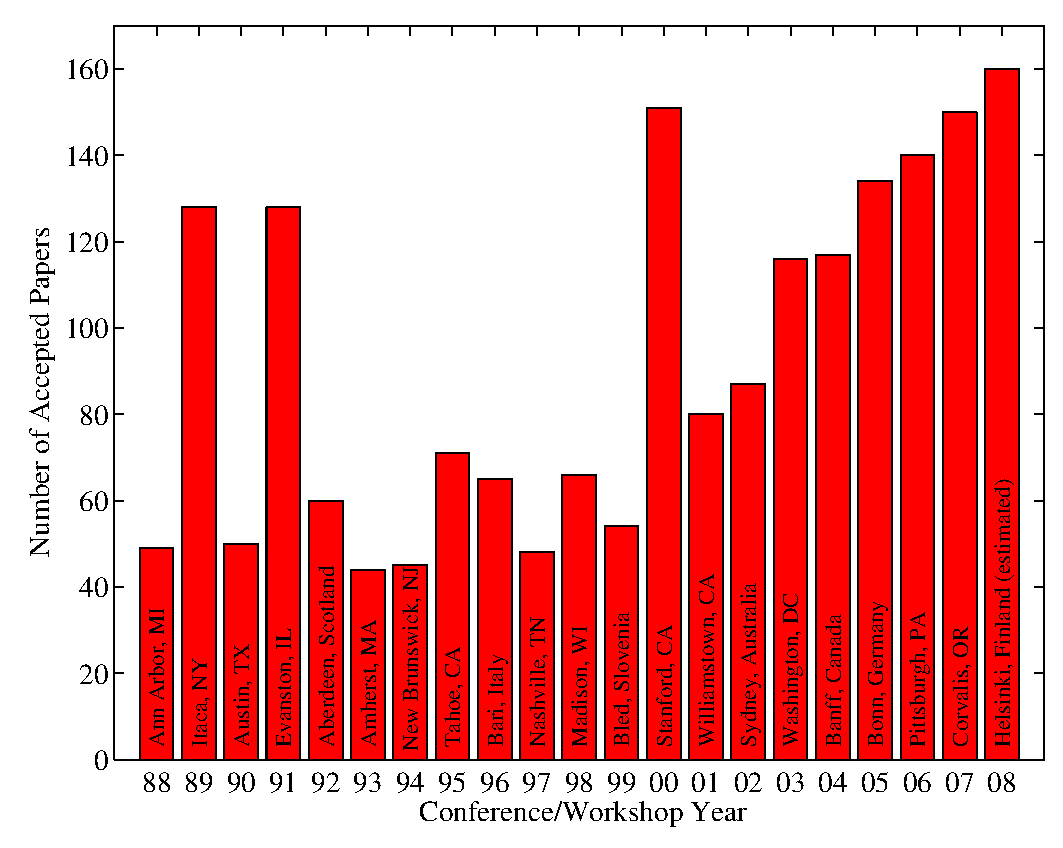
\includegraphics[width=\columnwidth]{figure/icml_numpapers.eps}}
\caption{Historical locations and number of accepted papers for International
Machine Learning Conferences (ICML 1993 -- ICML 2008) and International
Workshops on Machine Learning (ML 1988 -- ML 1992). At the time this figure was
produced, the number of accepted papers for ICML 2008 was unknown and instead
estimated.}
\label{icml-historical}
\end{center}
\vskip -0.2in
\end{figure}

\subsection{Figures}

You may want to include figures in the paper to illustrate
your approach and results. Such artwork should be centered,
legible, and separated from the text. Lines should be dark and at
least 0.5~points thick for purposes of reproduction, and text should
not appear on a gray background.

Label all distinct components of each figure. If the figure takes the
form of a graph, then give a name for each axis and include a legend
that briefly describes each curve. Do not include a title inside the
figure; instead, the caption should serve this function.

Number figures sequentially, placing the figure number and caption
\emph{after} the graphics, with at least 0.1~inches of space before
the caption and 0.1~inches after it, as in
\cref{icml-historical}. The figure caption should be set in
9~point type and centered unless it runs two or more lines, in which
case it should be flush left. You may float figures to the top or
bottom of a column, and you may set wide figures across both columns
(use the environment \texttt{figure*} in \LaTeX). Always place
two-column figures at the top or bottom of the page.

\subsection{Algorithms}

If you are using \LaTeX, please use the ``algorithm'' and ``algorithmic''
environments to format pseudocode. These require
the corresponding stylefiles, algorithm.sty and
algorithmic.sty, which are supplied with this package.
\cref{alg:example} shows an example.

\begin{algorithm}[tb]
   \caption{Bubble Sort}
   \label{alg:example}
\begin{algorithmic}
   \STATE {\bfseries Input:} data $x_i$, size $m$
   \REPEAT
   \STATE Initialize $noChange = true$.
   \FOR{$i=1$ {\bfseries to} $m-1$}
   \IF{$x_i > x_{i+1}$}
   \STATE Swap $x_i$ and $x_{i+1}$
   \STATE $noChange = false$
   \ENDIF
   \ENDFOR
   \UNTIL{$noChange$ is $true$}
\end{algorithmic}
\end{algorithm}

\subsection{Tables}

You may also want to include tables that summarize material. Like
figures, these should be centered, legible, and numbered consecutively.
However, place the title \emph{above} the table with at least
0.1~inches of space before the title and the same after it, as in
\cref{sample-table}. The table title should be set in 9~point
type and centered unless it runs two or more lines, in which case it
should be flush left.

% Note use of \abovespace and \belowspace to get reasonable spacing
% above and below tabular lines.

\begin{table}[t]
\caption{Classification accuracies for naive Bayes and flexible
Bayes on various data sets.}
\label{sample-table}
\vskip 0.15in
\begin{center}
\begin{small}
\begin{sc}
\begin{tabular}{lcccr}
\toprule
Data set & Naive & Flexible & Better? \\
\midrule
Breast    & 95.9$\pm$ 0.2& 96.7$\pm$ 0.2& $\surd$ \\
Cleveland & 83.3$\pm$ 0.6& 80.0$\pm$ 0.6& $\times$\\
Glass2    & 61.9$\pm$ 1.4& 83.8$\pm$ 0.7& $\surd$ \\
Credit    & 74.8$\pm$ 0.5& 78.3$\pm$ 0.6&         \\
Horse     & 73.3$\pm$ 0.9& 69.7$\pm$ 1.0& $\times$\\
Meta      & 67.1$\pm$ 0.6& 76.5$\pm$ 0.5& $\surd$ \\
Pima      & 75.1$\pm$ 0.6& 73.9$\pm$ 0.5&         \\
Vehicle   & 44.9$\pm$ 0.6& 61.5$\pm$ 0.4& $\surd$ \\
\bottomrule
\end{tabular}
\end{sc}
\end{small}
\end{center}
\vskip -0.1in
\end{table}

Tables contain textual material, whereas figures contain graphical material.
Specify the contents of each row and column in the table's topmost
row. Again, you may float tables to a column's top or bottom, and set
wide tables across both columns. Place two-column tables at the
top or bottom of the page.

\subsection{Theorems and such}
The preferred way is to number definitions, propositions, lemmas, etc. consecutively, within sections, as shown below.
\begin{definition}
\label{def:inj}
A function $f:X \to Y$ is injective if for any $x,y\in X$ different, $f(x)\ne f(y)$.
\end{definition}
Using \cref{def:inj} we immediate get the following result:
\begin{proposition}
If $f$ is injective mapping a set $X$ to another set $Y$, 
the cardinality of $Y$ is at least as large as that of $X$
\end{proposition}
\begin{proof} 
Left as an exercise to the reader. 
\end{proof}
\cref{lem:usefullemma} stated next will prove to be useful.
\begin{lemma}
\label{lem:usefullemma}
For any $f:X \to Y$ and $g:Y\to Z$ injective functions, $f \circ g$ is injective.
\end{lemma}
\begin{theorem}
\label{thm:bigtheorem}
If $f:X\to Y$ is bijective, the cardinality of $X$ and $Y$ are the same.
\end{theorem}
An easy corollary of \cref{thm:bigtheorem} is the following:
\begin{corollary}
If $f:X\to Y$ is bijective, 
the cardinality of $X$ is at least as large as that of $Y$.
\end{corollary}
\begin{assumption}
The set $X$ is finite.
\label{ass:xfinite}
\end{assumption}
\begin{remark}
According to some, it is only the finite case (cf. \cref{ass:xfinite}) that is interesting.
\end{remark}
%restatable

\subsection{Citations and References}

If you rely on the \LaTeX{} bibliographic
facility, use \texttt{natbib.sty}
included in the style-file package to obtain reference.

Citations within the text should include the authors' last names and
year. If the authors' names are included in the sentence, place only
the year in parentheses, for example when referencing Arthur Samuel's
pioneering work \yrcite{Samuel59}. Otherwise place the entire
reference in parentheses with the authors and year separated by a
comma \cite{Samuel59}. List multiple references separated by
semicolons \cite{kearns89,Samuel59,mitchell80}. Use the `et~al.'
construct only for citations with three or more authors or after
listing all authors to a publication in an earlier reference \cite{MachineLearningI}.

Use an unnumbered first-level section heading for the references, and use a
hanging indent style, with the first line of the reference flush against the
left margin and subsequent lines indented by 10 points. The references at the
end of this document give examples for journal articles \cite{Samuel59},
conference publications \cite{langley00}, book chapters \cite{Newell81}, books
\cite{DudaHart2nd}, edited volumes \cite{MachineLearningI}, technical reports
\cite{mitchell80}, and dissertations \cite{kearns89}.

Alphabetize references by the surnames of the first authors, with
single author entries preceding multiple author entries. Order
references for the same authors by year of publication, with the
earliest first. Make sure that each reference includes all relevant
information (e.g., page numbers).

Please put some effort into making references complete, presentable, and
consistent, e.g. use the actual current name of authors.
If using bibtex, please protect capital letters of names and
abbreviations in titles, for example, use \{B\}ayesian or \{L\}ipschitz
in your .bib file.
%
\section*{Acknowledgements}

Acknowledgements is an unnumbered section at the end of the paper. Typically, this will include thanks to colleagues who contributed to the ideas, and to funding agencies and corporate sponsors that provided financial support.
%\bibliographystyle{ACM-Reference-Format}


\bibliographystyle{abbrvnat}
\bibliography{ref}
%\printbibliography
%\newpage
%\appendix
%
\section{Output of run.sh}

sk5057@speech-rec-vm:~/kaldi/egs/tedlium/s5_r3$ ./run.sh
Stage 0 begin: downloading data
local/download_data.sh: downloading TEDLIUM_release-3 data (it won't re-download if it was already downloaded.)
--2022-02-27 16:02:17--  http://www.openslr.org/resources/51/TEDLIUM_release-3.tgz
Resolving www.openslr.org (www.openslr.org)... 46.101.158.64
Connecting to www.openslr.org (www.openslr.org)|46.101.158.64|:80... connected.
HTTP request sent, awaiting response... 302 Found
Location: https://us.openslr.org/resources/51/TEDLIUM_release-3.tgz [following]
--2022-02-27 16:02:18--  https://us.openslr.org/resources/51/TEDLIUM_release-3.tgz
Resolving us.openslr.org (us.openslr.org)... 46.101.158.64
Connecting to us.openslr.org (us.openslr.org)|46.101.158.64|:443... connected.
HTTP request sent, awaiting response... 200 OK
Length: 54320173876 (51G) [application/x-gzip]
Saving to: 'TEDLIUM_release-3.tgz'

TEDLIUM_release-3.tgz                           100%[=======================================================================================================>]  50.59G  26.4MB/s    in 32m 43s 

2022-02-27 16:35:01 (26.4 MB/s) - 'TEDLIUM_release-3.tgz' saved [54320173876/54320173876]

local/download_data.sh: extracting TEDLIUM_release-3 data
Stage 0 end: downloading data
----------------------- Stage 1 begin: prepare data ---------------------------
utils/validate_data_dir.sh: Successfully validated data-directory data/dev.orig
utils/validate_data_dir.sh: Successfully validated data-directory data/test.orig
extend_segment_times.py: extended 268263 segments; fixed 183022 overlapping segments
utils/validate_data_dir.sh: Successfully validated data-directory data/train.orig
utils/data/get_utt2dur.sh: data/dev.orig/utt2dur already exists with the expected length.  We won't recompute it.
utils/data/modify_speaker_info.sh: moving data/dev/cmvn.scp to data/dev/.backup/cmvn.scp
utils/data/modify_speaker_info.sh: copied data from data/dev.orig to data/dev, number of speakers changed from 8 to 38
utils/validate_data_dir.sh: Successfully validated data-directory data/dev
utils/data/get_utt2dur.sh: data/test.orig/utt2dur already exists with the expected length.  We won't recompute it.
utils/data/modify_speaker_info.sh: moving data/test/cmvn.scp to data/test/.backup/cmvn.scp
utils/data/modify_speaker_info.sh: copied data from data/test.orig to data/test, number of speakers changed from 11 to 59
utils/validate_data_dir.sh: Successfully validated data-directory data/test
utils/data/get_utt2dur.sh: data/train.orig/utt2dur already exists with the expected length.  We won't recompute it.
utils/data/modify_speaker_info.sh: copied data from data/train.orig to data/train, number of speakers changed from 2351 to 10334
utils/validate_data_dir.sh: Successfully validated data-directory data/train
----------------------- Stage 1 end: prepare data ---------------------------
----------------------- Stage 2 begin: prepare dict ---------------------------
Checking data/local/dict_nosp/silence_phones.txt ...
--> reading data/local/dict_nosp/silence_phones.txt
--> text seems to be UTF-8 or ASCII, checking whitespaces
--> text contains only allowed whitespaces
--> data/local/dict_nosp/silence_phones.txt is OK

Checking data/local/dict_nosp/optional_silence.txt ...
--> reading data/local/dict_nosp/optional_silence.txt
--> text seems to be UTF-8 or ASCII, checking whitespaces
--> text contains only allowed whitespaces
--> data/local/dict_nosp/optional_silence.txt is OK

Checking data/local/dict_nosp/nonsilence_phones.txt ...
--> reading data/local/dict_nosp/nonsilence_phones.txt
--> text seems to be UTF-8 or ASCII, checking whitespaces
--> text contains only allowed whitespaces
--> data/local/dict_nosp/nonsilence_phones.txt is OK

Checking disjoint: silence_phones.txt, nonsilence_phones.txt
--> disjoint property is OK.

Checking data/local/dict_nosp/lexicon.txt
--> reading data/local/dict_nosp/lexicon.txt
--> text seems to be UTF-8 or ASCII, checking whitespaces
--> text contains only allowed whitespaces
--> data/local/dict_nosp/lexicon.txt is OK

Checking data/local/dict_nosp/lexiconp.txt
--> reading data/local/dict_nosp/lexiconp.txt
--> text seems to be UTF-8 or ASCII, checking whitespaces
--> text contains only allowed whitespaces
--> data/local/dict_nosp/lexiconp.txt is OK

Checking lexicon pair data/local/dict_nosp/lexicon.txt and data/local/dict_nosp/lexiconp.txt
--> lexicon pair data/local/dict_nosp/lexicon.txt and data/local/dict_nosp/lexiconp.txt match

Checking data/local/dict_nosp/extra_questions.txt ...
--> data/local/dict_nosp/extra_questions.txt is empty (this is OK)
--> SUCCESS [validating dictionary directory data/local/dict_nosp]

----------------------- Stage 2 end: prepare dict ---------------------------
----------------------- Stage 2 begin: prepare lang ---------------------------
utils/prepare_lang.sh data/local/dict_nosp <unk> data/local/lang_nosp data/lang_nosp
Checking data/local/dict_nosp/silence_phones.txt ...
--> reading data/local/dict_nosp/silence_phones.txt
--> text seems to be UTF-8 or ASCII, checking whitespaces
--> text contains only allowed whitespaces
--> data/local/dict_nosp/silence_phones.txt is OK

Checking data/local/dict_nosp/optional_silence.txt ...
--> reading data/local/dict_nosp/optional_silence.txt
--> text seems to be UTF-8 or ASCII, checking whitespaces
--> text contains only allowed whitespaces
--> data/local/dict_nosp/optional_silence.txt is OK

Checking data/local/dict_nosp/nonsilence_phones.txt ...
--> reading data/local/dict_nosp/nonsilence_phones.txt
--> text seems to be UTF-8 or ASCII, checking whitespaces
--> text contains only allowed whitespaces
--> data/local/dict_nosp/nonsilence_phones.txt is OK

Checking disjoint: silence_phones.txt, nonsilence_phones.txt
--> disjoint property is OK.

Checking data/local/dict_nosp/lexicon.txt
--> reading data/local/dict_nosp/lexicon.txt
--> text seems to be UTF-8 or ASCII, checking whitespaces
--> text contains only allowed whitespaces
--> data/local/dict_nosp/lexicon.txt is OK

Checking data/local/dict_nosp/lexiconp.txt
--> reading data/local/dict_nosp/lexiconp.txt
--> text seems to be UTF-8 or ASCII, checking whitespaces
--> text contains only allowed whitespaces
--> data/local/dict_nosp/lexiconp.txt is OK

Checking lexicon pair data/local/dict_nosp/lexicon.txt and data/local/dict_nosp/lexiconp.txt
--> lexicon pair data/local/dict_nosp/lexicon.txt and data/local/dict_nosp/lexiconp.txt match

Checking data/local/dict_nosp/extra_questions.txt ...
--> data/local/dict_nosp/extra_questions.txt is empty (this is OK)
--> SUCCESS [validating dictionary directory data/local/dict_nosp]

fstaddselfloops data/lang_nosp/phones/wdisambig_phones.int data/lang_nosp/phones/wdisambig_words.int 
prepare_lang.sh: validating output directory
utils/validate_lang.pl data/lang_nosp
Checking existence of separator file
separator file data/lang_nosp/subword_separator.txt is empty or does not exist, deal in word case.
Checking data/lang_nosp/phones.txt ...
--> text seems to be UTF-8 or ASCII, checking whitespaces
--> text contains only allowed whitespaces
--> data/lang_nosp/phones.txt is OK

Checking words.txt: #0 ...
--> text seems to be UTF-8 or ASCII, checking whitespaces
--> text contains only allowed whitespaces
--> data/lang_nosp/words.txt is OK

Checking disjoint: silence.txt, nonsilence.txt, disambig.txt ...
--> silence.txt and nonsilence.txt are disjoint
--> silence.txt and disambig.txt are disjoint
--> disambig.txt and nonsilence.txt are disjoint
--> disjoint property is OK

Checking sumation: silence.txt, nonsilence.txt, disambig.txt ...
--> found no unexplainable phones in phones.txt

Checking data/lang_nosp/phones/context_indep.{txt, int, csl} ...
--> text seems to be UTF-8 or ASCII, checking whitespaces
--> text contains only allowed whitespaces
--> 10 entry/entries in data/lang_nosp/phones/context_indep.txt
--> data/lang_nosp/phones/context_indep.int corresponds to data/lang_nosp/phones/context_indep.txt
--> data/lang_nosp/phones/context_indep.csl corresponds to data/lang_nosp/phones/context_indep.txt
--> data/lang_nosp/phones/context_indep.{txt, int, csl} are OK

Checking data/lang_nosp/phones/nonsilence.{txt, int, csl} ...
--> text seems to be UTF-8 or ASCII, checking whitespaces
--> text contains only allowed whitespaces
--> 156 entry/entries in data/lang_nosp/phones/nonsilence.txt
--> data/lang_nosp/phones/nonsilence.int corresponds to data/lang_nosp/phones/nonsilence.txt
--> data/lang_nosp/phones/nonsilence.csl corresponds to data/lang_nosp/phones/nonsilence.txt
--> data/lang_nosp/phones/nonsilence.{txt, int, csl} are OK

Checking data/lang_nosp/phones/silence.{txt, int, csl} ...
--> text seems to be UTF-8 or ASCII, checking whitespaces
--> text contains only allowed whitespaces
--> 10 entry/entries in data/lang_nosp/phones/silence.txt
--> data/lang_nosp/phones/silence.int corresponds to data/lang_nosp/phones/silence.txt
--> data/lang_nosp/phones/silence.csl corresponds to data/lang_nosp/phones/silence.txt
--> data/lang_nosp/phones/silence.{txt, int, csl} are OK

Checking data/lang_nosp/phones/optional_silence.{txt, int, csl} ...
--> text seems to be UTF-8 or ASCII, checking whitespaces
--> text contains only allowed whitespaces
--> 1 entry/entries in data/lang_nosp/phones/optional_silence.txt
--> data/lang_nosp/phones/optional_silence.int corresponds to data/lang_nosp/phones/optional_silence.txt
--> data/lang_nosp/phones/optional_silence.csl corresponds to data/lang_nosp/phones/optional_silence.txt
--> data/lang_nosp/phones/optional_silence.{txt, int, csl} are OK

Checking data/lang_nosp/phones/disambig.{txt, int, csl} ...
--> text seems to be UTF-8 or ASCII, checking whitespaces
--> text contains only allowed whitespaces
--> 17 entry/entries in data/lang_nosp/phones/disambig.txt
--> data/lang_nosp/phones/disambig.int corresponds to data/lang_nosp/phones/disambig.txt
--> data/lang_nosp/phones/disambig.csl corresponds to data/lang_nosp/phones/disambig.txt
--> data/lang_nosp/phones/disambig.{txt, int, csl} are OK

Checking data/lang_nosp/phones/roots.{txt, int} ...
--> text seems to be UTF-8 or ASCII, checking whitespaces
--> text contains only allowed whitespaces
--> 41 entry/entries in data/lang_nosp/phones/roots.txt
--> data/lang_nosp/phones/roots.int corresponds to data/lang_nosp/phones/roots.txt
--> data/lang_nosp/phones/roots.{txt, int} are OK

Checking data/lang_nosp/phones/sets.{txt, int} ...
--> text seems to be UTF-8 or ASCII, checking whitespaces
--> text contains only allowed whitespaces
--> 41 entry/entries in data/lang_nosp/phones/sets.txt
--> data/lang_nosp/phones/sets.int corresponds to data/lang_nosp/phones/sets.txt
--> data/lang_nosp/phones/sets.{txt, int} are OK

Checking data/lang_nosp/phones/extra_questions.{txt, int} ...
--> text seems to be UTF-8 or ASCII, checking whitespaces
--> text contains only allowed whitespaces
--> 9 entry/entries in data/lang_nosp/phones/extra_questions.txt
--> data/lang_nosp/phones/extra_questions.int corresponds to data/lang_nosp/phones/extra_questions.txt
--> data/lang_nosp/phones/extra_questions.{txt, int} are OK

Checking data/lang_nosp/phones/word_boundary.{txt, int} ...
--> text seems to be UTF-8 or ASCII, checking whitespaces
--> text contains only allowed whitespaces
--> 166 entry/entries in data/lang_nosp/phones/word_boundary.txt
--> data/lang_nosp/phones/word_boundary.int corresponds to data/lang_nosp/phones/word_boundary.txt
--> data/lang_nosp/phones/word_boundary.{txt, int} are OK

Checking optional_silence.txt ...
--> reading data/lang_nosp/phones/optional_silence.txt
--> data/lang_nosp/phones/optional_silence.txt is OK

Checking disambiguation symbols: #0 and #1
--> data/lang_nosp/phones/disambig.txt has "#0" and "#1"
--> data/lang_nosp/phones/disambig.txt is OK

Checking topo ...

Checking word_boundary.txt: silence.txt, nonsilence.txt, disambig.txt ...
--> data/lang_nosp/phones/word_boundary.txt doesn't include disambiguation symbols
--> data/lang_nosp/phones/word_boundary.txt is the union of nonsilence.txt and silence.txt
--> data/lang_nosp/phones/word_boundary.txt is OK

Checking word-level disambiguation symbols...
--> data/lang_nosp/phones/wdisambig.txt exists (newer prepare_lang.sh)
Checking word_boundary.int and disambig.int
--> generating a 61 word/subword sequence
--> resulting phone sequence from L.fst corresponds to the word sequence
--> L.fst is OK
--> generating a 51 word/subword sequence
--> resulting phone sequence from L_disambig.fst corresponds to the word sequence
--> L_disambig.fst is OK

Checking data/lang_nosp/oov.{txt, int} ...
--> text seems to be UTF-8 or ASCII, checking whitespaces
--> text contains only allowed whitespaces
--> 1 entry/entries in data/lang_nosp/oov.txt
--> data/lang_nosp/oov.int corresponds to data/lang_nosp/oov.txt
--> data/lang_nosp/oov.{txt, int} are OK

--> data/lang_nosp/L.fst is olabel sorted
--> data/lang_nosp/L_disambig.fst is olabel sorted
--> data/lang_nosp/G.fst is ilabel sorted
--> data/lang_nosp/G.fst has 323671 states
fstdeterminizestar data/lang_nosp/G.fst /dev/null 
--> data/lang_nosp/G.fst is determinizable
--> utils/lang/check_g_properties.pl successfully validated data/lang_nosp/G.fst
--> utils/lang/check_g_properties.pl succeeded.
--> Testing determinizability of L_disambig . G
fstdeterminizestar 
fsttablecompose data/lang_nosp/L_disambig.fst data/lang_nosp/G.fst 
--> L_disambig . G is determinizable
--> SUCCESS [validating lang directory data/lang_nosp]
----------------------- Stage 2 end: prepare lang ---------------------------
----------------------- Stage 4 begin: lang model ---------------------------
local/ted_download_lm.sh: downloading Tedlium 4 gram language models (it won't re-download if it was already downloaded.)
--2022-02-27 16:54:07--  http://kaldi-asr.org/models/5/4gram_small.arpa.gz
Resolving kaldi-asr.org (kaldi-asr.org)... 46.101.158.64
Connecting to kaldi-asr.org (kaldi-asr.org)|46.101.158.64|:80... connected.
HTTP request sent, awaiting response... 416 Requested Range Not Satisfiable

    The file is already fully retrieved; nothing to do.

--2022-02-27 16:54:08--  http://kaldi-asr.org/models/5/4gram_big.arpa.gz
Resolving kaldi-asr.org (kaldi-asr.org)... 46.101.158.64
Connecting to kaldi-asr.org (kaldi-asr.org)|46.101.158.64|:80... connected.
HTTP request sent, awaiting response... 416 Requested Range Not Satisfiable

    The file is already fully retrieved; nothing to do.

----------------------- Stage 4 end: lang model ---------------------------
----------------------- Stage 5 begin---------------------------
local/format_lms.sh: not regenerating data/lang_nosp/G.fst as it already exists and 
.. is newer than the source LM.
arpa-to-const-arpa --bos-symbol=152215 --eos-symbol=152216 --unk-symbol=38 'gunzip -c data/local/local_lm/data/arpa/4gram_big.arpa.gz | utils/map_arpa_lm.pl data/lang_nosp_rescore/words.txt|' data/lang_nosp_rescore/G.carpa 
LOG (arpa-to-const-arpa[5.5.1009~1-e4940]:BuildConstArpaLm():const-arpa-lm.cc:1078) Reading gunzip -c data/local/local_lm/data/arpa/4gram_big.arpa.gz | utils/map_arpa_lm.pl data/lang_nosp_rescore/words.txt|
utils/map_arpa_lm.pl: Processing "\data\"
utils/map_arpa_lm.pl: Processing "\1-grams:\"
LOG (arpa-to-const-arpa[5.5.1009~1-e4940]:Read():arpa-file-parser.cc:94) Reading \data\ section.
LOG (arpa-to-const-arpa[5.5.1009~1-e4940]:Read():arpa-file-parser.cc:149) Reading \1-grams: section.
utils/map_arpa_lm.pl: Processing "\2-grams:\"
LOG (arpa-to-const-arpa[5.5.1009~1-e4940]:Read():arpa-file-parser.cc:149) Reading \2-grams: section.
utils/map_arpa_lm.pl: Processing "\3-grams:\"
LOG (arpa-to-const-arpa[5.5.1009~1-e4940]:Read():arpa-file-parser.cc:149) Reading \3-grams: section.
utils/map_arpa_lm.pl: Processing "\4-grams:\"
LOG (arpa-to-const-arpa[5.5.1009~1-e4940]:Read():arpa-file-parser.cc:149) Reading \4-grams: section.
local/format_lms.sh: not regenerating data/lang_nosp/G.fst as it already exists and 
.. is newer than the source LM.
local/format_lms.sh: not regenerating data/lang_nosp_rescore/ as it seems to already by up to date.
----------------------- Stage 5 end---------------------------
----------------------- Stage 6 begin---------------------------
steps/make_mfcc.sh --nj 30 --cmd run.pl data/test
steps/make_mfcc.sh: moving data/test/feats.scp to data/test/.backup
utils/validate_data_dir.sh: Successfully validated data-directory data/test
steps/make_mfcc.sh [info]: segments file exists: using that.
steps/make_mfcc.sh: Succeeded creating MFCC features for test
steps/compute_cmvn_stats.sh data/test
Succeeded creating CMVN stats for test
steps/make_mfcc.sh --nj 30 --cmd run.pl data/dev
steps/make_mfcc.sh: moving data/dev/feats.scp to data/dev/.backup
utils/validate_data_dir.sh: Successfully validated data-directory data/dev
steps/make_mfcc.sh [info]: segments file exists: using that.
steps/make_mfcc.sh: Succeeded creating MFCC features for dev
steps/compute_cmvn_stats.sh data/dev
Succeeded creating CMVN stats for dev
steps/make_mfcc.sh --nj 30 --cmd run.pl data/train
utils/validate_data_dir.sh: Successfully validated data-directory data/train
steps/make_mfcc.sh [info]: segments file exists: using that.
steps/make_mfcc.sh: It seems not all of the feature files were successfully procesed (268262 != 268263); consider using utils/fix_data_dir.sh data/train
steps/make_mfcc.sh: Succeeded creating MFCC features for train
steps/compute_cmvn_stats.sh data/train
Succeeded creating CMVN stats for train
----------------------- Stage 6 end---------------------------
----------------------- Stage 7 begin---------------------------
utils/subset_data_dir.sh: reducing #utt from 268263 to 10000
Reduced number of utterances from 10000 to 9135
Using fix_data_dir.sh to reconcile the other files.
fix_data_dir.sh: kept 9135 utterances out of 10000
utils/fix_data_dir.sh: filtered data/train_10kshort_nodup/cmvn.scp from 6125 to 5816 lines based on filter /tmp/kaldi.9HlN/speakers.
utils/fix_data_dir.sh: filtered data/train_10kshort_nodup/wav.scp from 2209 to 2190 lines based on filter /tmp/kaldi.9HlN/recordings.
utils/fix_data_dir.sh: filtered data/train_10kshort_nodup/reco2file_and_channel from 2209 to 2190 lines based on filter /tmp/kaldi.9HlN/recordings.
fix_data_dir.sh: old files are kept in data/train_10kshort_nodup/.backup
----------------------- Stage 7 end---------------------------
----------------------- Stage 8 begin---------------------------
steps/train_mono.sh --nj 20 --cmd run.pl data/train_10kshort_nodup data/lang_nosp exp/mono
filter_scps.pl: warning: some input lines were output to multiple files [OK if splitting per utt] 
filter_scps.pl: warning: some input lines were output to multiple files [OK if splitting per utt] 
steps/train_mono.sh: Initializing monophone system.
steps/train_mono.sh: Compiling training graphs
steps/train_mono.sh: Aligning data equally (pass 0)
steps/train_mono.sh: Pass 1
steps/train_mono.sh: Aligning data
steps/train_mono.sh: Pass 2
steps/train_mono.sh: Aligning data
steps/train_mono.sh: Pass 3
steps/train_mono.sh: Aligning data
steps/train_mono.sh: Pass 4
steps/train_mono.sh: Aligning data
steps/train_mono.sh: Pass 5
steps/train_mono.sh: Aligning data
steps/train_mono.sh: Pass 6
steps/train_mono.sh: Aligning data
steps/train_mono.sh: Pass 7
steps/train_mono.sh: Aligning data
steps/train_mono.sh: Pass 8
steps/train_mono.sh: Aligning data
steps/train_mono.sh: Pass 9
steps/train_mono.sh: Aligning data
steps/train_mono.sh: Pass 10
steps/train_mono.sh: Aligning data
steps/train_mono.sh: Pass 11
steps/train_mono.sh: Pass 12
steps/train_mono.sh: Aligning data
steps/train_mono.sh: Pass 13
steps/train_mono.sh: Pass 14
steps/train_mono.sh: Aligning data
steps/train_mono.sh: Pass 15
steps/train_mono.sh: Pass 16
steps/train_mono.sh: Aligning data
steps/train_mono.sh: Pass 17
steps/train_mono.sh: Pass 18
steps/train_mono.sh: Aligning data
steps/train_mono.sh: Pass 19
steps/train_mono.sh: Pass 20
steps/train_mono.sh: Aligning data
steps/train_mono.sh: Pass 21
steps/train_mono.sh: Pass 22
steps/train_mono.sh: Pass 23
steps/train_mono.sh: Aligning data
steps/train_mono.sh: Pass 24
steps/train_mono.sh: Pass 25
steps/train_mono.sh: Pass 26
steps/train_mono.sh: Aligning data
steps/train_mono.sh: Pass 27
steps/train_mono.sh: Pass 28
steps/train_mono.sh: Pass 29
steps/train_mono.sh: Aligning data
steps/train_mono.sh: Pass 30
steps/train_mono.sh: Pass 31
steps/train_mono.sh: Pass 32
steps/train_mono.sh: Aligning data
steps/train_mono.sh: Pass 33
steps/train_mono.sh: Pass 34
steps/train_mono.sh: Pass 35
steps/train_mono.sh: Aligning data
steps/train_mono.sh: Pass 36
steps/train_mono.sh: Pass 37
steps/train_mono.sh: Pass 38
steps/train_mono.sh: Aligning data
steps/train_mono.sh: Pass 39
steps/diagnostic/analyze_alignments.sh --cmd run.pl data/lang_nosp exp/mono
analyze_phone_length_stats.py: WARNING: optional-silence SIL is seen only 68.3287671233% of the time at utterance begin.  This may not be optimal.
analyze_phone_length_stats.py: WARNING: optional-silence SIL is seen only 72.9554922166% of the time at utterance end.  This may not be optimal.
steps/diagnostic/analyze_alignments.sh: see stats in exp/mono/log/analyze_alignments.log
2 warnings in exp/mono/log/analyze_alignments.log
4803 warnings in exp/mono/log/align.*.*.log
392 warnings in exp/mono/log/acc.*.*.log
exp/mono: nj=20 align prob=-95.91 over 3.10h [retry=1.9%, fail=0.1%] states=127 gauss=1001
steps/train_mono.sh: Done training monophone system in exp/mono
----------------------- Stage 8 end---------------------------
----------------------- Stage 9 begin---------------------------
steps/align_si.sh --nj 8 --cmd run.pl data/train data/lang_nosp exp/mono exp/mono_ali
** split_data.sh: warning, #lines is (utt2spk,feats.scp) is (268263,268262); you can 
**  use utils/fix_data_dir.sh data/train to fix this.
filter_scps.pl: warning: some input lines were output to multiple files [OK if splitting per utt] 
filter_scps.pl: warning: some input lines were output to multiple files [OK if splitting per utt] 
steps/align_si.sh: feature type is delta
steps/align_si.sh: aligning data in data/train using model from exp/mono, putting alignments in exp/mono_ali
steps/diagnostic/analyze_alignments.sh --cmd run.pl data/lang_nosp exp/mono_ali
steps/diagnostic/analyze_alignments.sh: see stats in exp/mono_ali/log/analyze_alignments.log
steps/align_si.sh: done aligning data.
steps/train_deltas.sh --cmd run.pl 2500 30000 data/train data/lang_nosp exp/mono_ali exp/tri1
** split_data.sh: warning, #lines is (utt2spk,feats.scp) is (268263,268262); you can 
**  use utils/fix_data_dir.sh data/train to fix this.
steps/train_deltas.sh: accumulating tree stats
steps/train_deltas.sh: getting questions for tree-building, via clustering
steps/train_deltas.sh: building the tree
steps/train_deltas.sh: converting alignments from exp/mono_ali to use current tree
steps/train_deltas.sh: compiling graphs of transcripts
steps/train_deltas.sh: training pass 1
steps/train_deltas.sh: training pass 2
steps/train_deltas.sh: training pass 3
steps/train_deltas.sh: training pass 4
steps/train_deltas.sh: training pass 5
steps/train_deltas.sh: training pass 6
steps/train_deltas.sh: training pass 7
steps/train_deltas.sh: training pass 8
steps/train_deltas.sh: training pass 9
steps/train_deltas.sh: training pass 10
steps/train_deltas.sh: aligning data
steps/train_deltas.sh: training pass 11
steps/train_deltas.sh: training pass 12
steps/train_deltas.sh: training pass 13
steps/train_deltas.sh: training pass 14
steps/train_deltas.sh: training pass 15
steps/train_deltas.sh: training pass 16
steps/train_deltas.sh: training pass 17
steps/train_deltas.sh: training pass 18
steps/train_deltas.sh: training pass 19
steps/train_deltas.sh: training pass 20
steps/train_deltas.sh: aligning data
steps/train_deltas.sh: training pass 21
steps/train_deltas.sh: training pass 22
steps/train_deltas.sh: training pass 23
steps/train_deltas.sh: training pass 24
steps/train_deltas.sh: training pass 25
steps/train_deltas.sh: training pass 26
steps/train_deltas.sh: training pass 27
steps/train_deltas.sh: training pass 28
steps/train_deltas.sh: training pass 29
steps/train_deltas.sh: training pass 30
steps/train_deltas.sh: aligning data
steps/train_deltas.sh: training pass 31
steps/train_deltas.sh: training pass 32
steps/train_deltas.sh: training pass 33
steps/train_deltas.sh: training pass 34
steps/diagnostic/analyze_alignments.sh --cmd run.pl data/lang_nosp exp/tri1
analyze_phone_length_stats.py: WARNING: optional-silence SIL is seen only 78.4632099505% of the time at utterance begin.  This may not be optimal.
steps/diagnostic/analyze_alignments.sh: see stats in exp/tri1/log/analyze_alignments.log
1 warnings in exp/tri1/log/build_tree.log
1 warnings in exp/tri1/log/analyze_alignments.log
52092 warnings in exp/tri1/log/align.*.*.log
35295 warnings in exp/tri1/log/acc.*.*.log
exp/tri1: nj=8 align prob=-96.38 over 448.23h [retry=6.0%, fail=0.5%] states=1960 gauss=30089 tree-impr=3.50
steps/train_deltas.sh: Done training system with delta+delta-delta features in exp/tri1
----------------------- Stage 9 end---------------------------
----------------------- Stage 10 begin---------------------------
tree-info exp/tri1/tree 
tree-info exp/tri1/tree 
fstdeterminizestar --use-log=true 
fstminimizeencoded 
fsttablecompose data/lang_nosp/L_disambig.fst data/lang_nosp/G.fst 
fstpushspecial 
WARNING (fstpushspecial[5.5.1009~1-e4940]:Iterate():push-special.cc:182) push-special: finished 200 iterations without converging.  Output will be inaccurate.
fstisstochastic data/lang_nosp/tmp/LG.fst 
-0.0965911 -0.162304
[info]: LG not stochastic.
fstcomposecontext --context-size=3 --central-position=1 --read-disambig-syms=data/lang_nosp/phones/disambig.int --write-disambig-syms=data/lang_nosp/tmp/disambig_ilabels_3_1.int data/lang_nosp/tmp/ilabels_3_1.30844 data/lang_nosp/tmp/LG.fst 
fstisstochastic data/lang_nosp/tmp/CLG_3_1.fst 
0 -0.162304
[info]: CLG not stochastic.
make-h-transducer --disambig-syms-out=exp/tri1/graph_nosp/disambig_tid.int --transition-scale=1.0 data/lang_nosp/tmp/ilabels_3_1 exp/tri1/tree exp/tri1/final.mdl 
fstdeterminizestar --use-log=true 
fsttablecompose exp/tri1/graph_nosp/Ha.fst data/lang_nosp/tmp/CLG_3_1.fst 
fstminimizeencoded 
fstrmsymbols exp/tri1/graph_nosp/disambig_tid.int 
fstrmepslocal 
fstisstochastic exp/tri1/graph_nosp/HCLGa.fst 
0.000488052 -0.310332
HCLGa is not stochastic
add-self-loops --self-loop-scale=0.1 --reorder=true exp/tri1/final.mdl exp/tri1/graph_nosp/HCLGa.fst 
steps/decode.sh --nj 8 --cmd run.pl --num-threads 4 exp/tri1/graph_nosp data/dev exp/tri1/decode_nosp_dev
filter_scps.pl: warning: some input lines were output to multiple files [OK if splitting per utt] 
filter_scps.pl: warning: some input lines were output to multiple files [OK if splitting per utt] 
decode.sh: feature type is delta
steps/diagnostic/analyze_lats.sh --cmd run.pl exp/tri1/graph_nosp exp/tri1/decode_nosp_dev
steps/diagnostic/analyze_lats.sh: see stats in exp/tri1/decode_nosp_dev/log/analyze_alignments.log
Overall, lattice depth (10,50,90-percentile)=(2,9,60) and mean=23.7
steps/diagnostic/analyze_lats.sh: see stats in exp/tri1/decode_nosp_dev/log/analyze_lattice_depth_stats.log
exp/tri1/decode_nosp_dev/wer_10
%WER 28.59 [ 5085 / 17783, 640 ins, 1189 del, 3256 sub ]
%SER 95.66 [ 485 / 507 ]
exp/tri1/decode_nosp_dev/wer_11
%WER 28.43 [ 5056 / 17783, 591 ins, 1269 del, 3196 sub ]
%SER 95.46 [ 484 / 507 ]
exp/tri1/decode_nosp_dev/wer_12
%WER 28.48 [ 5064 / 17783, 548 ins, 1369 del, 3147 sub ]
%SER 95.27 [ 483 / 507 ]
exp/tri1/decode_nosp_dev/wer_13
%WER 28.98 [ 5153 / 17783, 518 ins, 1457 del, 3178 sub ]
%SER 95.27 [ 483 / 507 ]
exp/tri1/decode_nosp_dev/wer_14
%WER 29.35 [ 5220 / 17783, 481 ins, 1538 del, 3201 sub ]
%SER 95.46 [ 484 / 507 ]
exp/tri1/decode_nosp_dev/wer_15
%WER 29.74 [ 5289 / 17783, 463 ins, 1619 del, 3207 sub ]
%SER 95.46 [ 484 / 507 ]
exp/tri1/decode_nosp_dev/wer_16
%WER 30.28 [ 5385 / 17783, 447 ins, 1691 del, 3247 sub ]
%SER 95.66 [ 485 / 507 ]
exp/tri1/decode_nosp_dev/wer_17
%WER 31.09 [ 5529 / 17783, 421 ins, 1803 del, 3305 sub ]
%SER 96.06 [ 487 / 507 ]
exp/tri1/decode_nosp_dev/wer_7
%WER 30.60 [ 5441 / 17783, 847 ins, 1014 del, 3580 sub ]
%SER 97.44 [ 494 / 507 ]
exp/tri1/decode_nosp_dev/wer_8
%WER 29.75 [ 5291 / 17783, 764 ins, 1073 del, 3454 sub ]
%SER 97.04 [ 492 / 507 ]
exp/tri1/decode_nosp_dev/wer_9
%WER 29.01 [ 5159 / 17783, 690 ins, 1128 del, 3341 sub ]
%SER 96.25 [ 488 / 507 ]
steps/lmrescore_const_arpa.sh --cmd run.pl data/lang_nosp data/lang_nosp_rescore data/dev exp/tri1/decode_nosp_dev exp/tri1/decode_nosp_dev_rescore
exp/tri1/decode_nosp_dev_rescore/wer_10
%WER 27.37 [ 4868 / 17783, 629 ins, 1174 del, 3065 sub ]
%SER 95.27 [ 483 / 507 ]
exp/tri1/decode_nosp_dev_rescore/wer_11
%WER 27.43 [ 4877 / 17783, 586 ins, 1257 del, 3034 sub ]
%SER 94.67 [ 480 / 507 ]
exp/tri1/decode_nosp_dev_rescore/wer_12
%WER 27.37 [ 4868 / 17783, 538 ins, 1333 del, 2997 sub ]
%SER 95.07 [ 482 / 507 ]
exp/tri1/decode_nosp_dev_rescore/wer_13
%WER 27.63 [ 4913 / 17783, 509 ins, 1412 del, 2992 sub ]
%SER 95.27 [ 483 / 507 ]
exp/tri1/decode_nosp_dev_rescore/wer_14
%WER 28.07 [ 4991 / 17783, 480 ins, 1498 del, 3013 sub ]
%SER 94.67 [ 480 / 507 ]
exp/tri1/decode_nosp_dev_rescore/wer_15
%WER 28.53 [ 5074 / 17783, 460 ins, 1573 del, 3041 sub ]
%SER 94.67 [ 480 / 507 ]
exp/tri1/decode_nosp_dev_rescore/wer_16
%WER 29.11 [ 5177 / 17783, 451 ins, 1670 del, 3056 sub ]
%SER 95.07 [ 482 / 507 ]
exp/tri1/decode_nosp_dev_rescore/wer_17
%WER 29.62 [ 5268 / 17783, 434 ins, 1739 del, 3095 sub ]
%SER 95.07 [ 482 / 507 ]
exp/tri1/decode_nosp_dev_rescore/wer_7
%WER 29.23 [ 5198 / 17783, 838 ins, 992 del, 3368 sub ]
%SER 95.86 [ 486 / 507 ]
exp/tri1/decode_nosp_dev_rescore/wer_8
%WER 28.31 [ 5035 / 17783, 750 ins, 1040 del, 3245 sub ]
%SER 96.25 [ 488 / 507 ]
exp/tri1/decode_nosp_dev_rescore/wer_9
%WER 27.44 [ 4880 / 17783, 669 ins, 1104 del, 3107 sub ]
%SER 96.06 [ 487 / 507 ]
steps/decode.sh --nj 8 --cmd run.pl --num-threads 4 exp/tri1/graph_nosp data/test exp/tri1/decode_nosp_test
filter_scps.pl: warning: some input lines were output to multiple files [OK if splitting per utt] 
filter_scps.pl: warning: some input lines were output to multiple files [OK if splitting per utt] 
decode.sh: feature type is delta
steps/diagnostic/analyze_lats.sh --cmd run.pl exp/tri1/graph_nosp exp/tri1/decode_nosp_test
steps/diagnostic/analyze_lats.sh: see stats in exp/tri1/decode_nosp_test/log/analyze_alignments.log
Overall, lattice depth (10,50,90-percentile)=(2,9,61) and mean=23.8
steps/diagnostic/analyze_lats.sh: see stats in exp/tri1/decode_nosp_test/log/analyze_lattice_depth_stats.log
exp/tri1/decode_nosp_test/wer_10
%WER 27.72 [ 7622 / 27500, 830 ins, 1574 del, 5218 sub ]
%SER 93.33 [ 1078 / 1155 ]
exp/tri1/decode_nosp_test/wer_11
%WER 27.62 [ 7596 / 27500, 761 ins, 1671 del, 5164 sub ]
%SER 92.81 [ 1072 / 1155 ]
exp/tri1/decode_nosp_test/wer_12
%WER 27.94 [ 7684 / 27500, 710 ins, 1791 del, 5183 sub ]
%SER 92.90 [ 1073 / 1155 ]
exp/tri1/decode_nosp_test/wer_13
%WER 28.30 [ 7783 / 27500, 661 ins, 1903 del, 5219 sub ]
%SER 92.99 [ 1074 / 1155 ]
exp/tri1/decode_nosp_test/wer_14
%WER 28.68 [ 7886 / 27500, 623 ins, 2032 del, 5231 sub ]
%SER 92.90 [ 1073 / 1155 ]
exp/tri1/decode_nosp_test/wer_15
%WER 29.25 [ 8045 / 27500, 588 ins, 2184 del, 5273 sub ]
%SER 93.16 [ 1076 / 1155 ]
exp/tri1/decode_nosp_test/wer_16
%WER 29.91 [ 8224 / 27500, 568 ins, 2295 del, 5361 sub ]
%SER 93.16 [ 1076 / 1155 ]
exp/tri1/decode_nosp_test/wer_17
%WER 30.67 [ 8435 / 27500, 548 ins, 2421 del, 5466 sub ]
%SER 93.68 [ 1082 / 1155 ]
exp/tri1/decode_nosp_test/wer_7
%WER 30.25 [ 8319 / 27500, 1166 ins, 1365 del, 5788 sub ]
%SER 93.77 [ 1083 / 1155 ]
exp/tri1/decode_nosp_test/wer_8
%WER 28.99 [ 7971 / 27500, 1028 ins, 1435 del, 5508 sub ]
%SER 93.42 [ 1079 / 1155 ]
exp/tri1/decode_nosp_test/wer_9
%WER 28.24 [ 7767 / 27500, 920 ins, 1509 del, 5338 sub ]
%SER 93.07 [ 1075 / 1155 ]
steps/lmrescore_const_arpa.sh --cmd run.pl data/lang_nosp data/lang_nosp_rescore data/test exp/tri1/decode_nosp_test exp/tri1/decode_nosp_test_rescore
exp/tri1/decode_nosp_test_rescore/wer_10
%WER 26.27 [ 7225 / 27500, 819 ins, 1498 del, 4908 sub ]
%SER 91.69 [ 1059 / 1155 ]
exp/tri1/decode_nosp_test_rescore/wer_11
%WER 26.32 [ 7237 / 27500, 763 ins, 1583 del, 4891 sub ]
%SER 91.43 [ 1056 / 1155 ]
exp/tri1/decode_nosp_test_rescore/wer_12
%WER 26.45 [ 7273 / 27500, 712 ins, 1672 del, 4889 sub ]
%SER 91.17 [ 1053 / 1155 ]
exp/tri1/decode_nosp_test_rescore/wer_13
%WER 26.72 [ 7349 / 27500, 666 ins, 1770 del, 4913 sub ]
%SER 91.52 [ 1057 / 1155 ]
exp/tri1/decode_nosp_test_rescore/wer_14
%WER 27.39 [ 7532 / 27500, 636 ins, 1887 del, 5009 sub ]
%SER 91.69 [ 1059 / 1155 ]
exp/tri1/decode_nosp_test_rescore/wer_15
%WER 27.97 [ 7692 / 27500, 599 ins, 2009 del, 5084 sub ]
%SER 91.95 [ 1062 / 1155 ]
exp/tri1/decode_nosp_test_rescore/wer_16
%WER 28.64 [ 7877 / 27500, 568 ins, 2134 del, 5175 sub ]
%SER 92.03 [ 1063 / 1155 ]
exp/tri1/decode_nosp_test_rescore/wer_17
%WER 29.30 [ 8058 / 27500, 554 ins, 2256 del, 5248 sub ]
%SER 92.21 [ 1065 / 1155 ]
exp/tri1/decode_nosp_test_rescore/wer_7
%WER 28.61 [ 7867 / 27500, 1127 ins, 1307 del, 5433 sub ]
%SER 93.51 [ 1080 / 1155 ]
exp/tri1/decode_nosp_test_rescore/wer_8
%WER 27.56 [ 7579 / 27500, 995 ins, 1374 del, 5210 sub ]
%SER 92.64 [ 1070 / 1155 ]
exp/tri1/decode_nosp_test_rescore/wer_9
%WER 26.70 [ 7343 / 27500, 889 ins, 1426 del, 5028 sub ]
%SER 91.60 [ 1058 / 1155 ]
----------------------- Stage 10 end---------------------------
----------------------- Stage 11 begin---------------------------
steps/align_si.sh --nj 8 --cmd run.pl data/train data/lang_nosp exp/tri1 exp/tri1_ali
steps/align_si.sh: feature type is delta
steps/align_si.sh: aligning data in data/train using model from exp/tri1, putting alignments in exp/tri1_ali
steps/diagnostic/analyze_alignments.sh --cmd run.pl data/lang_nosp exp/tri1_ali
analyze_phone_length_stats.py: WARNING: optional-silence SIL is seen only 78.1645154643% of the time at utterance begin.  This may not be optimal.
steps/diagnostic/analyze_alignments.sh: see stats in exp/tri1_ali/log/analyze_alignments.log
steps/align_si.sh: done aligning data.
steps/train_lda_mllt.sh --cmd run.pl 4000 50000 data/train data/lang_nosp exp/tri1_ali exp/tri2
** split_data.sh: warning, #lines is (utt2spk,feats.scp) is (268263,268262); you can 
**  use utils/fix_data_dir.sh data/train to fix this.
steps/train_lda_mllt.sh: Accumulating LDA statistics.
steps/train_lda_mllt.sh: Accumulating tree stats
steps/train_lda_mllt.sh: Getting questions for tree clustering.
steps/train_lda_mllt.sh: Building the tree
steps/train_lda_mllt.sh: Initializing the model
steps/train_lda_mllt.sh: Converting alignments from exp/tri1_ali to use current tree
steps/train_lda_mllt.sh: Compiling graphs of transcripts
Training pass 1
Training pass 2
steps/train_lda_mllt.sh: Estimating MLLT
Training pass 3
Training pass 4
steps/train_lda_mllt.sh: Estimating MLLT
Training pass 5
Training pass 6
steps/train_lda_mllt.sh: Estimating MLLT
Training pass 7
Training pass 8
Training pass 9
Training pass 10
Aligning data
Training pass 11
Training pass 12
steps/train_lda_mllt.sh: Estimating MLLT
Training pass 13
Training pass 14
Training pass 15
Training pass 16
Training pass 17
Training pass 18
Training pass 19
Training pass 20
Aligning data
Training pass 21
Training pass 22
Training pass 23
Training pass 24
Training pass 25
Training pass 26
Training pass 27
Training pass 28
Training pass 29
Training pass 30
Aligning data
Training pass 31
Training pass 32
Training pass 33
Training pass 34
steps/diagnostic/analyze_alignments.sh --cmd run.pl data/lang_nosp exp/tri2
analyze_phone_length_stats.py: WARNING: optional-silence SIL is seen only 76.467028961% of the time at utterance begin.  This may not be optimal.
analyze_phone_length_stats.py: WARNING: optional-silence SIL is seen only 78.0719260069% of the time at utterance end.  This may not be optimal.
steps/diagnostic/analyze_alignments.sh: see stats in exp/tri2/log/analyze_alignments.log
1 warnings in exp/tri2/log/build_tree.log
69374 warnings in exp/tri2/log/align.*.*.log
1357 warnings in exp/tri2/log/lda_acc.*.log
67603 warnings in exp/tri2/log/acc.*.*.log
2 warnings in exp/tri2/log/analyze_alignments.log
exp/tri2: nj=8 align prob=-49.45 over 446.63h [retry=7.3%, fail=0.8%] states=3280 gauss=50094 tree-impr=4.42 lda-sum=17.64 mllt:impr,logdet=0.90,1.45
steps/train_lda_mllt.sh: Done training system with LDA+MLLT features in exp/tri2
----------------------- Stage 11 end---------------------------
----------------------- Stage 12 begin---------------------------
tree-info exp/tri2/tree 
tree-info exp/tri2/tree 
make-h-transducer --disambig-syms-out=exp/tri2/graph_nosp/disambig_tid.int --transition-scale=1.0 data/lang_nosp/tmp/ilabels_3_1 exp/tri2/tree exp/tri2/final.mdl 
fstminimizeencoded 
fstrmsymbols exp/tri2/graph_nosp/disambig_tid.int 
fstrmepslocal 
fsttablecompose exp/tri2/graph_nosp/Ha.fst data/lang_nosp/tmp/CLG_3_1.fst 
fstdeterminizestar --use-log=true 
fstisstochastic exp/tri2/graph_nosp/HCLGa.fst 
0.000488052 -0.310332
HCLGa is not stochastic
add-self-loops --self-loop-scale=0.1 --reorder=true exp/tri2/final.mdl exp/tri2/graph_nosp/HCLGa.fst 
steps/decode.sh --nj 8 --cmd run.pl --num-threads 4 exp/tri2/graph_nosp data/dev exp/tri2/decode_nosp_dev
decode.sh: feature type is lda
steps/diagnostic/analyze_lats.sh --cmd run.pl exp/tri2/graph_nosp exp/tri2/decode_nosp_dev
steps/diagnostic/analyze_lats.sh: see stats in exp/tri2/decode_nosp_dev/log/analyze_alignments.log
Overall, lattice depth (10,50,90-percentile)=(1,5,32) and mean=13.2
steps/diagnostic/analyze_lats.sh: see stats in exp/tri2/decode_nosp_dev/log/analyze_lattice_depth_stats.log
exp/tri2/decode_nosp_dev/wer_10
%WER 25.24 [ 4489 / 17783, 704 ins, 939 del, 2846 sub ]
%SER 95.46 [ 484 / 507 ]
exp/tri2/decode_nosp_dev/wer_11
%WER 24.82 [ 4413 / 17783, 664 ins, 982 del, 2767 sub ]
%SER 95.07 [ 482 / 507 ]
exp/tri2/decode_nosp_dev/wer_12
%WER 24.51 [ 4358 / 17783, 602 ins, 1024 del, 2732 sub ]
%SER 95.07 [ 482 / 507 ]
exp/tri2/decode_nosp_dev/wer_13
%WER 24.53 [ 4362 / 17783, 577 ins, 1088 del, 2697 sub ]
%SER 95.07 [ 482 / 507 ]
exp/tri2/decode_nosp_dev/wer_14
%WER 24.52 [ 4361 / 17783, 559 ins, 1121 del, 2681 sub ]
%SER 94.67 [ 480 / 507 ]
exp/tri2/decode_nosp_dev/wer_15
%WER 24.48 [ 4353 / 17783, 535 ins, 1167 del, 2651 sub ]
%SER 94.87 [ 481 / 507 ]
exp/tri2/decode_nosp_dev/wer_16
%WER 24.78 [ 4406 / 17783, 515 ins, 1201 del, 2690 sub ]
%SER 95.07 [ 482 / 507 ]
exp/tri2/decode_nosp_dev/wer_17
%WER 25.06 [ 4456 / 17783, 497 ins, 1256 del, 2703 sub ]
%SER 95.07 [ 482 / 507 ]
exp/tri2/decode_nosp_dev/wer_7
%WER 27.63 [ 4913 / 17783, 888 ins, 833 del, 3192 sub ]
%SER 96.84 [ 491 / 507 ]
exp/tri2/decode_nosp_dev/wer_8
%WER 26.78 [ 4763 / 17783, 830 ins, 867 del, 3066 sub ]
%SER 95.86 [ 486 / 507 ]
exp/tri2/decode_nosp_dev/wer_9
%WER 25.81 [ 4589 / 17783, 753 ins, 900 del, 2936 sub ]
%SER 96.06 [ 487 / 507 ]
steps/lmrescore_const_arpa.sh --cmd run.pl data/lang_nosp data/lang_nosp_rescore data/dev exp/tri2/decode_nosp_dev exp/tri2/decode_nosp_dev_rescore
exp/tri2/decode_nosp_dev_rescore/wer_10
%WER 23.87 [ 4245 / 17783, 701 ins, 901 del, 2643 sub ]
%SER 94.48 [ 479 / 507 ]
exp/tri2/decode_nosp_dev_rescore/wer_11
%WER 23.37 [ 4155 / 17783, 644 ins, 942 del, 2569 sub ]
%SER 94.48 [ 479 / 507 ]
exp/tri2/decode_nosp_dev_rescore/wer_12
%WER 23.28 [ 4139 / 17783, 614 ins, 990 del, 2535 sub ]
%SER 94.48 [ 479 / 507 ]
exp/tri2/decode_nosp_dev_rescore/wer_13
%WER 23.21 [ 4127 / 17783, 586 ins, 1052 del, 2489 sub ]
%SER 94.48 [ 479 / 507 ]
exp/tri2/decode_nosp_dev_rescore/wer_14
%WER 23.16 [ 4119 / 17783, 552 ins, 1081 del, 2486 sub ]
%SER 93.69 [ 475 / 507 ]
exp/tri2/decode_nosp_dev_rescore/wer_15
%WER 23.31 [ 4146 / 17783, 540 ins, 1120 del, 2486 sub ]
%SER 93.89 [ 476 / 507 ]
exp/tri2/decode_nosp_dev_rescore/wer_16
%WER 23.54 [ 4186 / 17783, 521 ins, 1184 del, 2481 sub ]
%SER 94.08 [ 477 / 507 ]
exp/tri2/decode_nosp_dev_rescore/wer_17
%WER 23.73 [ 4220 / 17783, 505 ins, 1219 del, 2496 sub ]
%SER 93.89 [ 476 / 507 ]
exp/tri2/decode_nosp_dev_rescore/wer_7
%WER 26.43 [ 4700 / 17783, 874 ins, 811 del, 3015 sub ]
%SER 96.45 [ 489 / 507 ]
exp/tri2/decode_nosp_dev_rescore/wer_8
%WER 25.31 [ 4501 / 17783, 803 ins, 828 del, 2870 sub ]
%SER 95.66 [ 485 / 507 ]
exp/tri2/decode_nosp_dev_rescore/wer_9
%WER 24.63 [ 4380 / 17783, 756 ins, 871 del, 2753 sub ]
%SER 94.87 [ 481 / 507 ]
steps/decode.sh --nj 8 --cmd run.pl --num-threads 4 exp/tri2/graph_nosp data/test exp/tri2/decode_nosp_test
decode.sh: feature type is lda
steps/diagnostic/analyze_lats.sh --cmd run.pl exp/tri2/graph_nosp exp/tri2/decode_nosp_test
steps/diagnostic/analyze_lats.sh: see stats in exp/tri2/decode_nosp_test/log/analyze_alignments.log
Overall, lattice depth (10,50,90-percentile)=(1,5,33) and mean=13.8
steps/diagnostic/analyze_lats.sh: see stats in exp/tri2/decode_nosp_test/log/analyze_lattice_depth_stats.log
exp/tri2/decode_nosp_test/wer_10
%WER 24.24 [ 6667 / 27500, 896 ins, 1221 del, 4550 sub ]
%SER 91.52 [ 1057 / 1155 ]
exp/tri2/decode_nosp_test/wer_11
%WER 23.70 [ 6517 / 27500, 814 ins, 1285 del, 4418 sub ]
%SER 91.17 [ 1053 / 1155 ]
exp/tri2/decode_nosp_test/wer_12
%WER 23.49 [ 6460 / 27500, 758 ins, 1345 del, 4357 sub ]
%SER 90.91 [ 1050 / 1155 ]
exp/tri2/decode_nosp_test/wer_13
%WER 23.31 [ 6410 / 27500, 728 ins, 1400 del, 4282 sub ]
%SER 90.48 [ 1045 / 1155 ]
exp/tri2/decode_nosp_test/wer_14
%WER 23.40 [ 6434 / 27500, 693 ins, 1448 del, 4293 sub ]
%SER 90.56 [ 1046 / 1155 ]
exp/tri2/decode_nosp_test/wer_15
%WER 23.77 [ 6536 / 27500, 677 ins, 1530 del, 4329 sub ]
%SER 90.74 [ 1048 / 1155 ]
exp/tri2/decode_nosp_test/wer_16
%WER 24.11 [ 6631 / 27500, 669 ins, 1611 del, 4351 sub ]
%SER 90.74 [ 1048 / 1155 ]
exp/tri2/decode_nosp_test/wer_17
%WER 24.44 [ 6722 / 27500, 646 ins, 1684 del, 4392 sub ]
%SER 91.00 [ 1051 / 1155 ]
exp/tri2/decode_nosp_test/wer_7
%WER 27.27 [ 7500 / 27500, 1195 ins, 1090 del, 5215 sub ]
%SER 93.51 [ 1080 / 1155 ]
exp/tri2/decode_nosp_test/wer_8
%WER 26.02 [ 7155 / 27500, 1078 ins, 1134 del, 4943 sub ]
%SER 92.73 [ 1071 / 1155 ]
exp/tri2/decode_nosp_test/wer_9
%WER 24.96 [ 6865 / 27500, 982 ins, 1182 del, 4701 sub ]
%SER 92.38 [ 1067 / 1155 ]
steps/lmrescore_const_arpa.sh --cmd run.pl data/lang_nosp data/lang_nosp_rescore data/test exp/tri2/decode_nosp_test exp/tri2/decode_nosp_test_rescore
exp/tri2/decode_nosp_test_rescore/wer_10
%WER 22.64 [ 6226 / 27500, 864 ins, 1175 del, 4187 sub ]
%SER 90.74 [ 1048 / 1155 ]
exp/tri2/decode_nosp_test_rescore/wer_11
%WER 22.35 [ 6147 / 27500, 812 ins, 1246 del, 4089 sub ]
%SER 90.56 [ 1046 / 1155 ]
exp/tri2/decode_nosp_test_rescore/wer_12
%WER 22.01 [ 6053 / 27500, 758 ins, 1285 del, 4010 sub ]
%SER 90.30 [ 1043 / 1155 ]
exp/tri2/decode_nosp_test_rescore/wer_13
%WER 21.93 [ 6032 / 27500, 705 ins, 1325 del, 4002 sub ]
%SER 90.04 [ 1040 / 1155 ]
exp/tri2/decode_nosp_test_rescore/wer_14
%WER 21.96 [ 6039 / 27500, 677 ins, 1391 del, 3971 sub ]
%SER 89.61 [ 1035 / 1155 ]
exp/tri2/decode_nosp_test_rescore/wer_15
%WER 22.14 [ 6089 / 27500, 652 ins, 1446 del, 3991 sub ]
%SER 89.61 [ 1035 / 1155 ]
exp/tri2/decode_nosp_test_rescore/wer_16
%WER 22.39 [ 6157 / 27500, 625 ins, 1511 del, 4021 sub ]
%SER 89.70 [ 1036 / 1155 ]
exp/tri2/decode_nosp_test_rescore/wer_17
%WER 22.82 [ 6276 / 27500, 606 ins, 1581 del, 4089 sub ]
%SER 90.22 [ 1042 / 1155 ]
exp/tri2/decode_nosp_test_rescore/wer_7
%WER 25.83 [ 7103 / 27500, 1151 ins, 1099 del, 4853 sub ]
%SER 92.73 [ 1071 / 1155 ]
exp/tri2/decode_nosp_test_rescore/wer_8
%WER 24.67 [ 6784 / 27500, 1038 ins, 1124 del, 4622 sub ]
%SER 91.86 [ 1061 / 1155 ]
exp/tri2/decode_nosp_test_rescore/wer_9
%WER 23.48 [ 6458 / 27500, 936 ins, 1151 del, 4371 sub ]
%SER 90.91 [ 1050 / 1155 ]
----------------------- Stage 12 end---------------------------
----------------------- Stage 13 begin---------------------------
steps/get_prons.sh --cmd run.pl data/train data/lang_nosp exp/tri2
steps/get_prons.sh: exp/tri2/ali.1.gz exists, so starting from alignments.
steps/get_prons.sh: done writing prons to exp/tri2/prons.*.gz, silence counts in 
steps/get_prons.sh: exp/tri2/sil_counts_nowb.txt and pronunciation counts in 
steps/get_prons.sh: exp/tri2/pron_counts.{int,txt}
steps/get_prons.sh: ... and also in exp/tri2/pron_counts_nowb.txt
Checking data/local/dict_nosp/silence_phones.txt ...
--> reading data/local/dict_nosp/silence_phones.txt
--> text seems to be UTF-8 or ASCII, checking whitespaces
--> text contains only allowed whitespaces
--> data/local/dict_nosp/silence_phones.txt is OK

Checking data/local/dict_nosp/optional_silence.txt ...
--> reading data/local/dict_nosp/optional_silence.txt
--> text seems to be UTF-8 or ASCII, checking whitespaces
--> text contains only allowed whitespaces
--> data/local/dict_nosp/optional_silence.txt is OK

Checking data/local/dict_nosp/nonsilence_phones.txt ...
--> reading data/local/dict_nosp/nonsilence_phones.txt
--> text seems to be UTF-8 or ASCII, checking whitespaces
--> text contains only allowed whitespaces
--> data/local/dict_nosp/nonsilence_phones.txt is OK

Checking disjoint: silence_phones.txt, nonsilence_phones.txt
--> disjoint property is OK.

Checking data/local/dict_nosp/lexicon.txt
--> reading data/local/dict_nosp/lexicon.txt
--> text seems to be UTF-8 or ASCII, checking whitespaces
--> text contains only allowed whitespaces
--> data/local/dict_nosp/lexicon.txt is OK

Checking data/local/dict_nosp/lexiconp.txt
--> reading data/local/dict_nosp/lexiconp.txt
--> text seems to be UTF-8 or ASCII, checking whitespaces
--> text contains only allowed whitespaces
--> data/local/dict_nosp/lexiconp.txt is OK

Checking lexicon pair data/local/dict_nosp/lexicon.txt and data/local/dict_nosp/lexiconp.txt
--> lexicon pair data/local/dict_nosp/lexicon.txt and data/local/dict_nosp/lexiconp.txt match

Checking data/local/dict_nosp/extra_questions.txt ...
--> data/local/dict_nosp/extra_questions.txt is empty (this is OK)
--> SUCCESS [validating dictionary directory data/local/dict_nosp]

utils/dict_dir_add_pronprobs.sh: normalizing pronprobs so maximum is 1 for each word.
utils/dict_dir_add_pronprobs.sh: produced dictionary directory with probabilities in data/local/dict/
utils/dict_dir_add_pronprobs.sh: validating data/local/dict ..
Checking data/local/dict/silence_phones.txt ...
--> reading data/local/dict/silence_phones.txt
--> text seems to be UTF-8 or ASCII, checking whitespaces
--> text contains only allowed whitespaces
--> data/local/dict/silence_phones.txt is OK

Checking data/local/dict/optional_silence.txt ...
--> reading data/local/dict/optional_silence.txt
--> text seems to be UTF-8 or ASCII, checking whitespaces
--> text contains only allowed whitespaces
--> data/local/dict/optional_silence.txt is OK

Checking data/local/dict/nonsilence_phones.txt ...
--> reading data/local/dict/nonsilence_phones.txt
--> text seems to be UTF-8 or ASCII, checking whitespaces
--> text contains only allowed whitespaces
--> data/local/dict/nonsilence_phones.txt is OK

Checking disjoint: silence_phones.txt, nonsilence_phones.txt
--> disjoint property is OK.

Checking data/local/dict/lexicon.txt
--> reading data/local/dict/lexicon.txt
--> text seems to be UTF-8 or ASCII, checking whitespaces
--> text contains only allowed whitespaces
--> data/local/dict/lexicon.txt is OK

Checking data/local/dict/lexiconp.txt
--> reading data/local/dict/lexiconp.txt
--> text seems to be UTF-8 or ASCII, checking whitespaces
--> text contains only allowed whitespaces
--> data/local/dict/lexiconp.txt is OK

Checking data/local/dict/lexiconp_silprob.txt
--> reading data/local/dict/lexiconp_silprob.txt
--> text seems to be UTF-8 or ASCII, checking whitespaces
--> text contains only allowed whitespaces
--> data/local/dict/lexiconp_silprob.txt is OK

Checking lexicon pair data/local/dict/lexicon.txt and data/local/dict/lexiconp.txt
--> lexicon pair data/local/dict/lexicon.txt and data/local/dict/lexiconp.txt match

Checking lexicon pair data/local/dict/lexiconp.txt and data/local/dict/lexiconp_silprob.txt
--> lexicon pair data/local/dict/lexiconp.txt and data/local/dict/lexiconp_silprob.txt match

Checking data/local/dict/extra_questions.txt ...
--> data/local/dict/extra_questions.txt is empty (this is OK)
--> SUCCESS [validating dictionary directory data/local/dict]

Some low-probability prons include: 
# sort -k2,2 -n data/local/dict/lexiconp.txt  | head -n 8
family 0.00358423 F AE M AE L IY
eventually 0.00431965 IY V EH N CH AH W AH L IY
beyond 0.00548446 B IH AO N D
beyond 0.00731261 B IH AA N D
destruction 0.00735294 D AE S T R AH K SH AE N
vaccine 0.00806452 V AA CH IY N
american 0.00843373 AE M EH R AE K AE N
actually 0.00937735 AE K CH AH W AH L IY
----------------------- Stage 13 end---------------------------
----------------------- Stage 14 begin---------------------------
utils/prepare_lang.sh data/local/dict <unk> data/local/lang data/lang
Checking data/local/dict/silence_phones.txt ...
--> reading data/local/dict/silence_phones.txt
--> text seems to be UTF-8 or ASCII, checking whitespaces
--> text contains only allowed whitespaces
--> data/local/dict/silence_phones.txt is OK

Checking data/local/dict/optional_silence.txt ...
--> reading data/local/dict/optional_silence.txt
--> text seems to be UTF-8 or ASCII, checking whitespaces
--> text contains only allowed whitespaces
--> data/local/dict/optional_silence.txt is OK

Checking data/local/dict/nonsilence_phones.txt ...
--> reading data/local/dict/nonsilence_phones.txt
--> text seems to be UTF-8 or ASCII, checking whitespaces
--> text contains only allowed whitespaces
--> data/local/dict/nonsilence_phones.txt is OK

Checking disjoint: silence_phones.txt, nonsilence_phones.txt
--> disjoint property is OK.

Checking data/local/dict/lexicon.txt
--> reading data/local/dict/lexicon.txt
--> text seems to be UTF-8 or ASCII, checking whitespaces
--> text contains only allowed whitespaces
--> data/local/dict/lexicon.txt is OK

Checking data/local/dict/lexiconp.txt
--> reading data/local/dict/lexiconp.txt
--> text seems to be UTF-8 or ASCII, checking whitespaces
--> text contains only allowed whitespaces
--> data/local/dict/lexiconp.txt is OK

Checking data/local/dict/lexiconp_silprob.txt
--> reading data/local/dict/lexiconp_silprob.txt
--> text seems to be UTF-8 or ASCII, checking whitespaces
--> text contains only allowed whitespaces
--> data/local/dict/lexiconp_silprob.txt is OK

Checking lexicon pair data/local/dict/lexicon.txt and data/local/dict/lexiconp.txt
--> lexicon pair data/local/dict/lexicon.txt and data/local/dict/lexiconp.txt match

Checking lexicon pair data/local/dict/lexiconp.txt and data/local/dict/lexiconp_silprob.txt
--> lexicon pair data/local/dict/lexiconp.txt and data/local/dict/lexiconp_silprob.txt match

Checking data/local/dict/extra_questions.txt ...
--> data/local/dict/extra_questions.txt is empty (this is OK)
--> SUCCESS [validating dictionary directory data/local/dict]

fstaddselfloops data/lang/phones/wdisambig_phones.int data/lang/phones/wdisambig_words.int 
prepare_lang.sh: validating output directory
utils/validate_lang.pl data/lang
Checking existence of separator file
separator file data/lang/subword_separator.txt is empty or does not exist, deal in word case.
Checking data/lang/phones.txt ...
--> text seems to be UTF-8 or ASCII, checking whitespaces
--> text contains only allowed whitespaces
--> data/lang/phones.txt is OK

Checking words.txt: #0 ...
--> text seems to be UTF-8 or ASCII, checking whitespaces
--> text contains only allowed whitespaces
--> data/lang/words.txt is OK

Checking disjoint: silence.txt, nonsilence.txt, disambig.txt ...
--> silence.txt and nonsilence.txt are disjoint
--> silence.txt and disambig.txt are disjoint
--> disambig.txt and nonsilence.txt are disjoint
--> disjoint property is OK

Checking sumation: silence.txt, nonsilence.txt, disambig.txt ...
--> found no unexplainable phones in phones.txt

Checking data/lang/phones/context_indep.{txt, int, csl} ...
--> text seems to be UTF-8 or ASCII, checking whitespaces
--> text contains only allowed whitespaces
--> 10 entry/entries in data/lang/phones/context_indep.txt
--> data/lang/phones/context_indep.int corresponds to data/lang/phones/context_indep.txt
--> data/lang/phones/context_indep.csl corresponds to data/lang/phones/context_indep.txt
--> data/lang/phones/context_indep.{txt, int, csl} are OK

Checking data/lang/phones/nonsilence.{txt, int, csl} ...
--> text seems to be UTF-8 or ASCII, checking whitespaces
--> text contains only allowed whitespaces
--> 156 entry/entries in data/lang/phones/nonsilence.txt
--> data/lang/phones/nonsilence.int corresponds to data/lang/phones/nonsilence.txt
--> data/lang/phones/nonsilence.csl corresponds to data/lang/phones/nonsilence.txt
--> data/lang/phones/nonsilence.{txt, int, csl} are OK

Checking data/lang/phones/silence.{txt, int, csl} ...
--> text seems to be UTF-8 or ASCII, checking whitespaces
--> text contains only allowed whitespaces
--> 10 entry/entries in data/lang/phones/silence.txt
--> data/lang/phones/silence.int corresponds to data/lang/phones/silence.txt
--> data/lang/phones/silence.csl corresponds to data/lang/phones/silence.txt
--> data/lang/phones/silence.{txt, int, csl} are OK

Checking data/lang/phones/optional_silence.{txt, int, csl} ...
--> text seems to be UTF-8 or ASCII, checking whitespaces
--> text contains only allowed whitespaces
--> 1 entry/entries in data/lang/phones/optional_silence.txt
--> data/lang/phones/optional_silence.int corresponds to data/lang/phones/optional_silence.txt
--> data/lang/phones/optional_silence.csl corresponds to data/lang/phones/optional_silence.txt
--> data/lang/phones/optional_silence.{txt, int, csl} are OK

Checking data/lang/phones/disambig.{txt, int, csl} ...
--> text seems to be UTF-8 or ASCII, checking whitespaces
--> text contains only allowed whitespaces
--> 17 entry/entries in data/lang/phones/disambig.txt
--> data/lang/phones/disambig.int corresponds to data/lang/phones/disambig.txt
--> data/lang/phones/disambig.csl corresponds to data/lang/phones/disambig.txt
--> data/lang/phones/disambig.{txt, int, csl} are OK

Checking data/lang/phones/roots.{txt, int} ...
--> text seems to be UTF-8 or ASCII, checking whitespaces
--> text contains only allowed whitespaces
--> 41 entry/entries in data/lang/phones/roots.txt
--> data/lang/phones/roots.int corresponds to data/lang/phones/roots.txt
--> data/lang/phones/roots.{txt, int} are OK

Checking data/lang/phones/sets.{txt, int} ...
--> text seems to be UTF-8 or ASCII, checking whitespaces
--> text contains only allowed whitespaces
--> 41 entry/entries in data/lang/phones/sets.txt
--> data/lang/phones/sets.int corresponds to data/lang/phones/sets.txt
--> data/lang/phones/sets.{txt, int} are OK

Checking data/lang/phones/extra_questions.{txt, int} ...
--> text seems to be UTF-8 or ASCII, checking whitespaces
--> text contains only allowed whitespaces
--> 9 entry/entries in data/lang/phones/extra_questions.txt
--> data/lang/phones/extra_questions.int corresponds to data/lang/phones/extra_questions.txt
--> data/lang/phones/extra_questions.{txt, int} are OK

Checking data/lang/phones/word_boundary.{txt, int} ...
--> text seems to be UTF-8 or ASCII, checking whitespaces
--> text contains only allowed whitespaces
--> 166 entry/entries in data/lang/phones/word_boundary.txt
--> data/lang/phones/word_boundary.int corresponds to data/lang/phones/word_boundary.txt
--> data/lang/phones/word_boundary.{txt, int} are OK

Checking optional_silence.txt ...
--> reading data/lang/phones/optional_silence.txt
--> data/lang/phones/optional_silence.txt is OK

Checking disambiguation symbols: #0 and #1
--> data/lang/phones/disambig.txt has "#0" and "#1"
--> data/lang/phones/disambig.txt is OK

Checking topo ...

Checking word_boundary.txt: silence.txt, nonsilence.txt, disambig.txt ...
--> data/lang/phones/word_boundary.txt doesn't include disambiguation symbols
--> data/lang/phones/word_boundary.txt is the union of nonsilence.txt and silence.txt
--> data/lang/phones/word_boundary.txt is OK

Checking word-level disambiguation symbols...
--> data/lang/phones/wdisambig.txt exists (newer prepare_lang.sh)
Checking word_boundary.int and disambig.int
--> generating a 25 word/subword sequence
--> resulting phone sequence from L.fst corresponds to the word sequence
--> L.fst is OK
--> generating a 99 word/subword sequence
--> resulting phone sequence from L_disambig.fst corresponds to the word sequence
--> L_disambig.fst is OK

Checking data/lang/oov.{txt, int} ...
--> text seems to be UTF-8 or ASCII, checking whitespaces
--> text contains only allowed whitespaces
--> 1 entry/entries in data/lang/oov.txt
--> data/lang/oov.int corresponds to data/lang/oov.txt
--> data/lang/oov.{txt, int} are OK

--> data/lang/L.fst is olabel sorted
--> data/lang/L_disambig.fst is olabel sorted
--> SUCCESS [validating lang directory data/lang]
tree-info exp/tri2/tree 
tree-info exp/tri2/tree 
fstminimizeencoded 
fstdeterminizestar --use-log=true 
fstpushspecial 
fsttablecompose data/lang/L_disambig.fst data/lang/G.fst 
WARNING (fstpushspecial[5.5.1009~1-e4940]:Iterate():push-special.cc:182) push-special: finished 200 iterations without converging.  Output will be inaccurate.
fstisstochastic data/lang/tmp/LG.fst 
-0.0590792 -0.0951427
[info]: LG not stochastic.
fstcomposecontext --context-size=3 --central-position=1 --read-disambig-syms=data/lang/phones/disambig.int --write-disambig-syms=data/lang/tmp/disambig_ilabels_3_1.int data/lang/tmp/ilabels_3_1.18225 data/lang/tmp/LG.fst 
fstisstochastic data/lang/tmp/CLG_3_1.fst 
0 -0.0951427
[info]: CLG not stochastic.
make-h-transducer --disambig-syms-out=exp/tri2/graph/disambig_tid.int --transition-scale=1.0 data/lang/tmp/ilabels_3_1 exp/tri2/tree exp/tri2/final.mdl 
fsttablecompose exp/tri2/graph/Ha.fst data/lang/tmp/CLG_3_1.fst 
fstdeterminizestar --use-log=true 
fstminimizeencoded 
fstrmsymbols exp/tri2/graph/disambig_tid.int 
fstrmepslocal 
fstisstochastic exp/tri2/graph/HCLGa.fst 
0.000488016 -0.215253
HCLGa is not stochastic
add-self-loops --self-loop-scale=0.1 --reorder=true exp/tri2/final.mdl exp/tri2/graph/HCLGa.fst 
steps/decode.sh --nj 8 --cmd run.pl --num-threads 4 exp/tri2/graph data/dev exp/tri2/decode_dev
decode.sh: feature type is lda
steps/diagnostic/analyze_lats.sh --cmd run.pl exp/tri2/graph exp/tri2/decode_dev
steps/diagnostic/analyze_lats.sh: see stats in exp/tri2/decode_dev/log/analyze_alignments.log
Overall, lattice depth (10,50,90-percentile)=(1,5,30) and mean=12.7
steps/diagnostic/analyze_lats.sh: see stats in exp/tri2/decode_dev/log/analyze_lattice_depth_stats.log
exp/tri2/decode_dev/wer_10
%WER 24.79 [ 4408 / 17783, 756 ins, 840 del, 2812 sub ]
%SER 95.07 [ 482 / 507 ]
exp/tri2/decode_dev/wer_11
%WER 24.34 [ 4329 / 17783, 699 ins, 878 del, 2752 sub ]
%SER 95.27 [ 483 / 507 ]
exp/tri2/decode_dev/wer_12
%WER 23.74 [ 4221 / 17783, 656 ins, 894 del, 2671 sub ]
%SER 94.87 [ 481 / 507 ]
exp/tri2/decode_dev/wer_13
%WER 23.57 [ 4192 / 17783, 641 ins, 920 del, 2631 sub ]
%SER 94.48 [ 479 / 507 ]
exp/tri2/decode_dev/wer_14
%WER 23.49 [ 4178 / 17783, 622 ins, 954 del, 2602 sub ]
%SER 94.28 [ 478 / 507 ]
exp/tri2/decode_dev/wer_15
%WER 23.48 [ 4176 / 17783, 601 ins, 974 del, 2601 sub ]
%SER 94.48 [ 479 / 507 ]
exp/tri2/decode_dev/wer_16
%WER 23.57 [ 4192 / 17783, 584 ins, 1023 del, 2585 sub ]
%SER 94.28 [ 478 / 507 ]
exp/tri2/decode_dev/wer_17
%WER 23.69 [ 4212 / 17783, 567 ins, 1062 del, 2583 sub ]
%SER 94.28 [ 478 / 507 ]
exp/tri2/decode_dev/wer_7
%WER 27.50 [ 4890 / 17783, 960 ins, 750 del, 3180 sub ]
%SER 97.04 [ 492 / 507 ]
exp/tri2/decode_dev/wer_8
%WER 26.23 [ 4664 / 17783, 883 ins, 763 del, 3018 sub ]
%SER 96.06 [ 487 / 507 ]
exp/tri2/decode_dev/wer_9
%WER 25.27 [ 4493 / 17783, 797 ins, 806 del, 2890 sub ]
%SER 95.46 [ 484 / 507 ]
steps/lmrescore_const_arpa.sh --cmd run.pl data/lang data/lang_rescore data/dev exp/tri2/decode_dev exp/tri2/decode_dev_rescore
exp/tri2/decode_dev_rescore/wer_10
%WER 23.19 [ 4123 / 17783, 740 ins, 800 del, 2583 sub ]
%SER 94.67 [ 480 / 507 ]
exp/tri2/decode_dev_rescore/wer_11
%WER 22.51 [ 4003 / 17783, 683 ins, 818 del, 2502 sub ]
%SER 94.08 [ 477 / 507 ]
exp/tri2/decode_dev_rescore/wer_12
%WER 22.33 [ 3971 / 17783, 663 ins, 848 del, 2460 sub ]
%SER 93.69 [ 475 / 507 ]
exp/tri2/decode_dev_rescore/wer_13
%WER 22.19 [ 3946 / 17783, 631 ins, 876 del, 2439 sub ]
%SER 93.69 [ 475 / 507 ]
exp/tri2/decode_dev_rescore/wer_14
%WER 22.14 [ 3937 / 17783, 613 ins, 911 del, 2413 sub ]
%SER 93.69 [ 475 / 507 ]
exp/tri2/decode_dev_rescore/wer_15
%WER 22.26 [ 3959 / 17783, 598 ins, 950 del, 2411 sub ]
%SER 93.69 [ 475 / 507 ]
exp/tri2/decode_dev_rescore/wer_16
%WER 22.20 [ 3948 / 17783, 584 ins, 983 del, 2381 sub ]
%SER 93.10 [ 472 / 507 ]
exp/tri2/decode_dev_rescore/wer_17
%WER 22.43 [ 3988 / 17783, 571 ins, 1010 del, 2407 sub ]
%SER 93.10 [ 472 / 507 ]
exp/tri2/decode_dev_rescore/wer_7
%WER 26.00 [ 4623 / 17783, 919 ins, 741 del, 2963 sub ]
%SER 95.86 [ 486 / 507 ]
exp/tri2/decode_dev_rescore/wer_8
%WER 24.68 [ 4389 / 17783, 837 ins, 737 del, 2815 sub ]
%SER 95.66 [ 485 / 507 ]
exp/tri2/decode_dev_rescore/wer_9
%WER 23.93 [ 4255 / 17783, 781 ins, 786 del, 2688 sub ]
%SER 95.07 [ 482 / 507 ]
steps/decode.sh --nj 8 --cmd run.pl --num-threads 4 exp/tri2/graph data/test exp/tri2/decode_test
decode.sh: feature type is lda
steps/diagnostic/analyze_lats.sh --cmd run.pl exp/tri2/graph exp/tri2/decode_test
steps/diagnostic/analyze_lats.sh: see stats in exp/tri2/decode_test/log/analyze_alignments.log
Overall, lattice depth (10,50,90-percentile)=(1,5,31) and mean=13.2
steps/diagnostic/analyze_lats.sh: see stats in exp/tri2/decode_test/log/analyze_lattice_depth_stats.log
exp/tri2/decode_test/wer_10
%WER 23.51 [ 6465 / 27500, 966 ins, 1053 del, 4446 sub ]
%SER 91.00 [ 1051 / 1155 ]
exp/tri2/decode_test/wer_11
%WER 22.82 [ 6275 / 27500, 894 ins, 1082 del, 4299 sub ]
%SER 90.82 [ 1049 / 1155 ]
exp/tri2/decode_test/wer_12
%WER 22.41 [ 6163 / 27500, 832 ins, 1112 del, 4219 sub ]
%SER 90.22 [ 1042 / 1155 ]
exp/tri2/decode_test/wer_13
%WER 22.29 [ 6130 / 27500, 774 ins, 1174 del, 4182 sub ]
%SER 90.48 [ 1045 / 1155 ]
exp/tri2/decode_test/wer_14
%WER 22.23 [ 6113 / 27500, 746 ins, 1202 del, 4165 sub ]
%SER 90.22 [ 1042 / 1155 ]
exp/tri2/decode_test/wer_15
%WER 22.38 [ 6155 / 27500, 717 ins, 1259 del, 4179 sub ]
%SER 90.13 [ 1041 / 1155 ]
exp/tri2/decode_test/wer_16
%WER 22.62 [ 6220 / 27500, 701 ins, 1311 del, 4208 sub ]
%SER 90.48 [ 1045 / 1155 ]
exp/tri2/decode_test/wer_17
%WER 22.93 [ 6306 / 27500, 687 ins, 1373 del, 4246 sub ]
%SER 90.56 [ 1046 / 1155 ]
exp/tri2/decode_test/wer_7
%WER 26.69 [ 7341 / 27500, 1275 ins, 973 del, 5093 sub ]
%SER 93.33 [ 1078 / 1155 ]
exp/tri2/decode_test/wer_8
%WER 25.07 [ 6895 / 27500, 1130 ins, 987 del, 4778 sub ]
%SER 92.64 [ 1070 / 1155 ]
exp/tri2/decode_test/wer_9
%WER 23.99 [ 6598 / 27500, 1029 ins, 1012 del, 4557 sub ]
%SER 91.60 [ 1058 / 1155 ]
steps/lmrescore_const_arpa.sh --cmd run.pl data/lang data/lang_rescore data/test exp/tri2/decode_test exp/tri2/decode_test_rescore
exp/tri2/decode_test_rescore/wer_10
%WER 21.95 [ 6035 / 27500, 878 ins, 1015 del, 4142 sub ]
%SER 89.96 [ 1039 / 1155 ]
exp/tri2/decode_test_rescore/wer_11
%WER 21.59 [ 5936 / 27500, 838 ins, 1051 del, 4047 sub ]
%SER 89.78 [ 1037 / 1155 ]
exp/tri2/decode_test_rescore/wer_12
%WER 21.28 [ 5851 / 27500, 802 ins, 1078 del, 3971 sub ]
%SER 90.04 [ 1040 / 1155 ]
exp/tri2/decode_test_rescore/wer_13
%WER 21.13 [ 5810 / 27500, 757 ins, 1118 del, 3935 sub ]
%SER 89.61 [ 1035 / 1155 ]
exp/tri2/decode_test_rescore/wer_14
%WER 21.12 [ 5809 / 27500, 717 ins, 1154 del, 3938 sub ]
%SER 89.52 [ 1034 / 1155 ]
exp/tri2/decode_test_rescore/wer_15
%WER 21.21 [ 5834 / 27500, 703 ins, 1184 del, 3947 sub ]
%SER 89.70 [ 1036 / 1155 ]
exp/tri2/decode_test_rescore/wer_16
%WER 21.30 [ 5858 / 27500, 686 ins, 1228 del, 3944 sub ]
%SER 89.44 [ 1033 / 1155 ]
exp/tri2/decode_test_rescore/wer_17
%WER 21.57 [ 5931 / 27500, 679 ins, 1275 del, 3977 sub ]
%SER 89.52 [ 1034 / 1155 ]
exp/tri2/decode_test_rescore/wer_7
%WER 25.16 [ 6918 / 27500, 1227 ins, 953 del, 4738 sub ]
%SER 92.03 [ 1063 / 1155 ]
exp/tri2/decode_test_rescore/wer_8
%WER 23.89 [ 6571 / 27500, 1089 ins, 960 del, 4522 sub ]
%SER 91.34 [ 1055 / 1155 ]
exp/tri2/decode_test_rescore/wer_9
%WER 22.80 [ 6271 / 27500, 988 ins, 986 del, 4297 sub ]
%SER 90.56 [ 1046 / 1155 ]
----------------------- Stage 14 end---------------------------
----------------------- Stage 15 begin---------------------------
steps/align_si.sh --nj 8 --cmd run.pl data/train data/lang exp/tri2 exp/tri2_ali
steps/align_si.sh: feature type is lda
steps/align_si.sh: aligning data in data/train using model from exp/tri2, putting alignments in exp/tri2_ali
steps/diagnostic/analyze_alignments.sh --cmd run.pl data/lang exp/tri2_ali
steps/diagnostic/analyze_alignments.sh: see stats in exp/tri2_ali/log/analyze_alignments.log
steps/align_si.sh: done aligning data.
steps/train_sat.sh --cmd run.pl 5000 100000 data/train data/lang exp/tri2_ali exp/tri3
steps/train_sat.sh: feature type is lda
steps/train_sat.sh: obtaining initial fMLLR transforms since not present in exp/tri2_ali
steps/train_sat.sh: Accumulating tree stats
steps/train_sat.sh: Getting questions for tree clustering.
steps/train_sat.sh: Building the tree
steps/train_sat.sh: Initializing the model
steps/train_sat.sh: Converting alignments from exp/tri2_ali to use current tree
steps/train_sat.sh: Compiling graphs of transcripts
Pass 1
Pass 2
Estimating fMLLR transforms
Pass 3
Pass 4
Estimating fMLLR transforms
Pass 5
Pass 6
Estimating fMLLR transforms




\end{document}